%% Copyright 2023 P. S. Eduardo.
%
% This work may be distributed and/or modified under the
% conditions of the LaTeX Project Public License, either version 1.3
% of this license or (at your option) any later version.
% 
% The Current Maintainer of this work is P. S. Eduardo.
%
% This work consists of the file poli.cls.
%% -----------------------------------------------------------------
% Escola Politécnica UFRJ LaTeX Template
% Version: 2302
% Author: Eduardo Paiva dos Santos
% email: eduardopaiva@poli.ufrj.br
% Base: CoppeTeX 2.3
%%------------------------------------------------------------------
\documentclass[grad,pdftex]{poli}
\usepackage[utf8]{inputenc}
\usepackage{amsmath,amssymb}
\usepackage{float}
\usepackage{multirow}
\usepackage{longtable}
\usepackage{tikz}
\usetikzlibrary{shapes,arrows,chains,positioning}
\usepackage{enumitem}
\usepackage{indentfirst}
\usepackage{array}
\usepackage{diagbox}
\usepackage[T1]{fontenc}
\usepackage{lipsum}
\usepackage[style=abnt-numeric, backend=biber]{biblatex} % Estilo ABNT e citações numéricas
\usepackage{listings}
\usepackage{acronym} 
\usepackage[ruled,vlined,portuguese]{algorithm2e}
\usepackage{hyperref}

\addbibresource{thesis.bib} % Arquivo .bib contendo as referências
\setcounter{secnumdepth}{4}

\lstset{
  language=Python,
  basicstyle=\ttfamily\small,
  keywordstyle=\color{blue},
  commentstyle=\color{green!40!black},
  stringstyle=\color{red},
  showstringspaces=false,
  breaklines=true,
  frame=single
}

\DeclareCiteCommand{\cite}[\mkbibbrackets]
  {\usebibmacro{cite:init}%
   \usebibmacro{prenote}}%
  {\usebibmacro{citeindex}%
   \usebibmacro{cite:comp}}%
  {\iftoggle{comp}{}{\multicitedelim}}%
  {\usebibmacro{cite:dump}%
   \usebibmacro{postnote}}%

\DeclareCiteCommand{\parencite}[\mkbibbrackets]%
  {\usebibmacro{cite:init}%
   \usebibmacro{prenote}}%
  {\usebibmacro{citeindex}%
   \usebibmacro{cite:comp}}%
  {\iftoggle{comp}{}{\multicitedelim}}%
  {\usebibmacro{cite:dump}%
\usebibmacro{postnote}}%

\makeatletter
  \renewbibmacro*{textcite}{% >>>3
    \iftoggle{comp}{%
      \iffieldequals{namehash}{\cbx@lasthash}%
        {\usebibmacro{cite:comp}}%
        {\usebibmacro{cite:dump}%
        \ifbool{cbx:parens}%
          {\printtext{\bibclosebracket}\global\boolfalse{cbx:parens}}%
          {}%
        \iffirstcitekey%
          {}%
          {\textcitedelim}%
        \usebibmacro{cite:init}%
        \printtext[bibhyperref]{%
          \ifnameundef{labelname}%
            {\printfield[citetitle]{labeltitle}}%
            {\printnames{labelname}}%
        }
        \setunit*{\printdelim{namelabeldelim}}%
        \printtext{\bibopenbracket}\global\booltrue{cbx:parens}%
        \ifnumequal{\value{citecount}}{1}%
          {\usebibmacro{prenote}}%
          {}%
        \usebibmacro{cite:comp}%
        \stepcounter{textcitecount}%
        \savefield{namehash}{\cbx@lasthash}}%
    }{%
      \iffieldequals{namehash}{\cbx@lasthash}%
            {\setunit{\multicitedelim}}%
            {\printtext[bibhyperref]{%
              \ifnameundef{labelname}%
                {\printfield[citetitle]{labeltitle}}%
                {\printnames{labelname}
             }}%
            \setunit*{\printdelim{namelabeldelim}}%
            \printtext{\bibopenbracket}\global\booltrue{cbx:parens}%
            \stepcounter{textcitecount}%
            \savefield{namehash}{\cbx@lasthash}}%
          \ifnumequal{\value{citecount}}{1}%
            {\usebibmacro{prenote}}%
            {}%
          \usebibmacro{cite}%
          \setunit{%
            \ifbool{cbx:parens}%
              {\bibclosebracket\global\boolfalse{cbx:parens}}%
              {}%
            \textcitedelim}%
    }%
}%

  \renewbibmacro*{textcite:postnote}{%
    \usebibmacro{postnote}%
    \ifthenelse{\value{multicitecount}=\value{multicitetotal}}%
      {\setunit{}%
      \printtext{%
        \ifbool{cbx:parens}%
          {\bibclosebracket\global\boolfalse{cbx:parens}}%
          {}}}%
      {\setunit{%
        \ifbool{cbx:parens}%
          {\bibclosebracket\global\boolfalse{cbx:parens}}%
          {}%
        \textcitedelim}}}%

  \DeclareCiteCommand{\cbx@textcite}%
    {\iftoggle{comp}{\usebibmacro{cite:init}}{\usebibmacro{textcite:init}}}%
    {\usebibmacro{citeindex}%
    \usebibmacro{textcite}}%
    {}%
    {\iftoggle{comp}{%
      \usebibmacro{cite:dump}%
          \usebibmacro{postnote}%
          \ifbool{cbx:parens}%
            {\bibclosebracket\global\boolfalse{cbx:parens}}%
            {}%
    }{%
      \usebibmacro{textcite:postnote}%
}}%
\makeatother



\DeclareFieldFormat{labelnumberwidth}{\mkbibbrackets{#1}}

\begin{document}
\title{Controle preditivo baseado em Deep Learning de geometria de cordão simples fundido por Manufatura Aditiva Arco Elétrico}
\foreigntitle{Deep Learning-based Predictive control of Wire+Arc Additive Manufacturing single bead geometry}
\author{Lucas}{Costa Barbosa}
\advisor{Prof.}{Fernando}{Cesar Lizarralde}{D.Sc.}
%\coadvisor{Prof.}{Nome}{Sobrenome}{D.Sc.}
\examiner{Prof.}{Nome Completo}{Ph.D.}
\examiner{Prof.}{Nome Completo}{D.Sc.}
%\examiner{Prof.}{Nome Completo}{D.Sc.}
\department{DEE} %UTTILIZE A SIGLA DO SEU DEPARTAMENTO MODIFICAR OS NOMES DE CURSO, DEPARTAMENTO E OBTENÇÃO DE GRAU (Obs: caso tenha algum equívoco nesses argumentos, necessário modificar o arquivo poli.cls no local que faz a leitura deste argumento)
\maketitle

\frontmatter
\chapter*{Agradecimentos}

Agradeço aos meus pais por todo o apoio e investimento na minha formação, e a todos aqueles que tem alguma parte nesse trabalho, especialmente os professores e colegas de curso. Aproveito para agradecer também a todos os amigos que me aturam até hoje e que não poderão mais fazer piada com o fato de eu não ter me formado.
\begin{abstract}
Apresenta-se neste trabalho uma aplicação de Rede Neural capaz de estimar em tempo real as características geométricas (largura e altura) de cordões simples fabricados através da Manufatura Aditivo por Arco de Arame (WAAM). 

A área da Manufatura Aditiva (MA), vêm se tornando cada vez mais estudada e desenvolvida no contexto da Indústria 4.0 por conta da sua capacidade de produzir peças com geometrias complexas, reduzido uso de material, e propriedades mecânicas superiores (os chamados metamateriais). 

No entanto, no contexto de WAAM as dinâmicas físicas do processo ainda são pouco conhecidas, devido a alta complexidade de modelagem, fazendo com que as peças não apresentem conformação e uniformidade geométrica. Para contornar problema são utilizados modelos aproximados que não necessariamente possuem uma boa razão performance - complexidade.

Com isso, alguns estudos utilizam modelos de \textit{Deep Learning} (DL), as chamadas Rede Neurais (RN), para estimar as características geométricas do cordão (altura e largura) baseado nos parâmetros de solda (como corrente, tensão e velocidade de alimentação do arame). A arquitetura utilizada foi a \textit{Long-Short Term Memory} (LSTM), que foi acoplada a uma malha de fechada de controle funcionando como um controlador.
\end{abstract}


\begin{foreignabstract}
This work presents a Neural Network application capable of estimating in real time the geometric characteristics (width and height) of simple strands manufactured through Wire Arc Additive Manufacturing (WAAM).

The area of Additive Manufacturing (AM) has become increasingly studied and developed in the context of Industry 4.0 due to its ability to produce parts with complex geometries, reduced material use, and superior mechanical properties (the so-called metamaterials).

However, in the context of WAAM, the physical dynamics of the process are still little known, due to the high complexity of modeling, causing the parts to lack conformation and geometric uniformity. To work around this problem, approximate models are used that do not necessarily have a good performance-complexity ratio.

As a result, some studies use Deep Learning (DL) models, the so-called Neural Networks (RN), to estimate the geometric characteristics of the bead (height and width) based on welding parameters (such as current, voltage and wire feed speed). The architecture used was Long-Short Term Memory (LSTM) network, which was coupled to a closed control loop working as a controller.
\end{foreignabstract}


\tableofcontents
\listoffigures
\listoftables
\chapter{Lista de Abreviações}
\begin{acronym}[] % Give the longest label here so that the list is nicely aligned
    \acro{CNC}{Controle Numérico Computadorizado}
    \acro{CNN}{Rede Neural Convolucional}
    \acro{DDP}{\textit{Direct Deposit Parameters}}
    \acro{GMAW}{\textit{Gas Metal Arc Weld}}
    \acro{GTAW}{\textit{Gas Tungsten Arc Weld}}
    \acro{IDP}{\textit{Indirect Deposit Parameters}}
    \acro{LSTM}{\textit{Long-Short Term Memory}}
    \acro{MA}{Manufatura Aditiva}
    \acro{ML}{\textit{Machine Learning}}
    \acro{MLP}{\textit{Multi Layer Perceptron}}
    \acro{MPC}{\textit{Model Predictive Control}}
    \acro{PAW}{\textit{Plasma Arc Weld}}
    \acro{RNN}{Rede Neural Recorrente}
    \acro{STL}{\textit{Standard Tessellation Language}}
    \acro{TS}{\textit{Travel Speed}}
    \acro{WAAM}{\textit{Wire+Arc Additive Manufacturing}}
    \acro{WFS}{\textit{Wire Feed Speed}}
\end{acronym}

\mainmatter
% \chapter{Introdução}
No contexto da Indústria 4.0, o setor fabril testemunhou grandes avanços no desenvolvimento da Manufatura Aditiva (MA), que permite a fabricação de peças de geometrias complexas com grandes liberdades de design e reduzido gasto de material e tempo (40-60\% do tempo de fabricação e 15-20\% do tempo de pós processamento). A MA tem se estabelecido como uma das mais promissoras tecnologias na indústria moderna. Entre suas diversas modalidades, destaca-se a Manufatura Aditiva por Arco e Arame (WAAM - Wire Arc Additive Manufacturing), uma técnica que vem ganhando crescente atenção e aplicação em diversos setores industriais, através do uso de manipuladores robóticos modernos. Um sistema básico de MA consiste na combinação de um sistema de movimento, uma fonte de calor e um material usado para a formar a peça fabricada. No caso de WAAM, o manipulador é encarregado da trajetória, a fonte é responsável por fundir o arame, o material usado para a fabricação das peças, geralmente ligas de Titânio, Alumínio ou Aço.\cite{williams2016wire, wu2018review}. 

A utilização de técnicas de MA como a WAAM se diferem das demais na capacidade de produzir peças de grandes dimensões como peças de aviões e foguetes, que possuem uma geometria não trivial. Porém, apresentam-se diversos riscos ao processo, devido a grande quantidade de calor absorvida pela peça, levando a deformações causadas pela tensão residual acumulada e um acabamento insatisfatório, como camadas de cordões sem uma uniformidade geométrica (altura e largura constantes) \cite{ding2015wire}.

A inspeção é uma etapa fundamental do processo, ajudando na detecção de defeitos e aumentando a confiança no produto final. Porém, além de ser uma tarefa não trivial, a avaliação de qualidade do produto não é suficiente para dar conta de todos as possíveis falhas de fabricação. Com isso, torna-se necessário o desenvolvimento de um sistema que seja capaz de controlar de forma eficiente as características geométricas da peça fabricada por WAAM. Este trabalho foca no desenvolvimento de uma Rede Neural (RN) capaz de identificar a dinâmica não linear e complexa do processo de impressão via WAAM, estimando as características geométricas (altura e largura) do cordão de solda a partir das séries temporais de parâmetros de solda da fabricação e da configuração do robô (Corrente e Velocidade de Alimentação de Arame (\textit{Wire Feed Speed} - WFS), utilizando a arquitetura das redes de Memória de Curto-Longo Prazo (\textit{Long Short Term Memory} - LSTM). Posteriormente, essa RN é utilizada como modelo dentro de um controlador MPC, com o objetivo de criar um sistema de controle inteligente.

\section{Motivação}
Com o desenvolvimento e modernização cada vez mais acelerada dos processos fabris, sistemas de MA como WAAM serão protagonistas na fabricação de peças complexas para os setores da aviação e aeroespacial, por exemplo. Com isso, é de extrema importância e urgência que sejam desenvolvidos sistemas inteligentes para controle da fabricação das peças através dessa técnica, com o intuito de melhorar sua qualidade. Para isso, é necessário desenvolver modelos capazes de identificar a dinâmica não linear do processo, mapeando os parâmetros de solda às características geométricas resultantes, para que seja possível fechar a malha de controle do sistema inteligente de WAAM. Portanto, o desenvolvimento da RN abordada neste trabalho é relevante já que não há um modelo consolidado na indústria capaz de realizar esta tarefa nos dias de hoje.

\section{Objetivos}
O objetivo deste trabalho é criar uma rede LSTM capaz de estimar os parâmetros geométricas de cordão único a partir da série temporal dos parâmetros de soldagem, modelando a dinâmica não linear do processo GMAW. Ademais, a rede será utilizada juntamente com um otimizador quadrático como modelo dentro uma malha de controle preditivo, criando assim um sistema de inteligente de controle da geometria da peça.
% \chapter{Revisão Bibliográfica}
\label{chap2}

\section{Manufatura Aditiva}

A Manufatura Aditiva (MA) é um processo de fabricação totalmente customizado, através da impressão em três dimensões de uma peça cuja geometria foi projetada em algum software de modelagem CAD (\textit{Computer-Aided Design}). Diferente da Manufatura Subtrativa, onde retira-se parte do material para se chegar na peça, na MA acontece a sobreposição de camadas deste material, que são unidas através de diferentes processos \cite{gibson2021additive}. A tecnologia começou sendo utilizada para fabricação de peças poliméricos e cerâmicos, sendo depois expandida para outros materiais como ligas metálicas para peças para a indústria, que se interessou pelas vantagens de redução de custos e tempo de fabricação, bem como a possibilidade de fabricar peças com geometrias complexas. A fabricação em MA consiste, basicamente, na deposição gradual de um material camada a camada \cite{srinivas2017critical}. Este material é aquecido através de um sistema de aquecimento e depositado por algum sistema robótico cuja trajetória é computadorizada, os chamados sistemas CNC (Controle Numérico Computadorizado). O fluxo da fabricação via MA é ilustrado na figura \ref{fig:ma_steps}:
\newpage
\begin{figure}[hbt!]
    \centering
    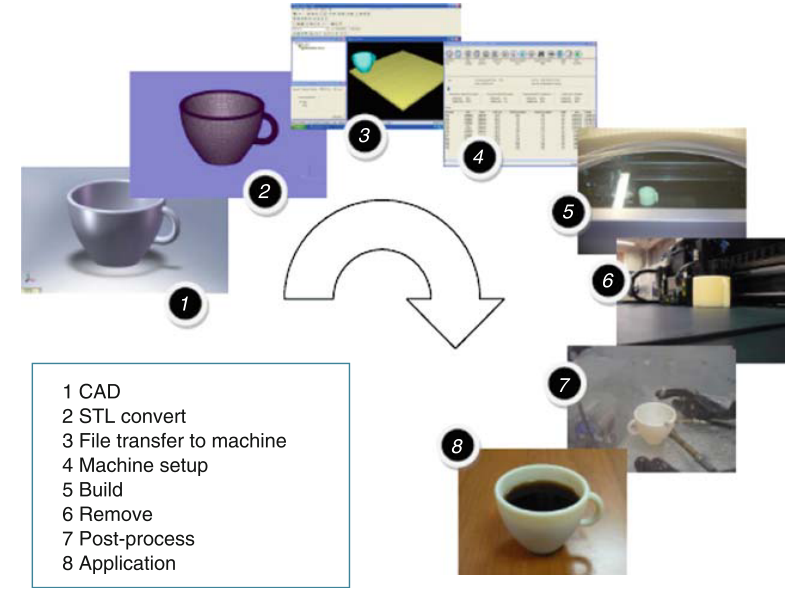
\includegraphics[width=0.8\linewidth]{Imagens/chap02/ma_steps.png}
    \caption{Etapas do processo de MA \cite{gibson2021additive}.}
    \label{fig:ma_steps}
\end{figure}
\begin{enumerate}[start=0]
    \item Seleção da técnica e material: Dependendo da aplicação, uma técnica e material correspondentes são mais recomendados. A técnica e o material influenciarâo nas demais etapas (ex: peças fabricadas por SLM não podem possuir regiões vazias totalmente internas, pois o pó não teria por onde escapar.

    \item Modelagem em CAD: Esta etapa consiste na modelagem de uma geometria tridimensional que compreende totalmente a superfície externa de um objeto.

    \item Conversão para arquivo STL: O arquivo STL contém toda a informação a respeito da superfície geométrica criada em CAD.

    \item Transferência do arquivo para a máquina de MA (Fatiamento): O arquivo necessita ser transferido para máquina para que ela o manipule, ajeitando posicionamento, tamanho e direcionamento.

    \item Configuração da máquina: Antes da fabricação, é necessário configurar alguns parâmetros para otimizar o resultado, tais como  a espessura da camada, a fonte de energia e o tempo de fabricação.
    
    \item Fabricação: Esta etapa é gerenciada automaticamente pela máquina. Só é necessário um monitoramento superficial para assegurar de que ainda há material, se a impressão está indo bem, etc.

    \item Remoção: Após a fabricação, é necessário remover a peça da máquina. Algumas máquinas possuem mecanismos de segurança que impedem a sua abertura até que a temperatura esfrie até um determinado valor.

    \item Pós-processamento: Algumas peças necessitam de acabamento, como limpeza e remoção de suportes de impressão ou tratamento térmico.

    \item Aplicação: Depois de todos esses processos, a peça está pronta para ser aplicada.
\end{enumerate}

As empresas que utilizam a MA possuem diferencial competitiva ao possuírem reduzidos custos e tempo de fabricação, maior facilidade em atender restrições ambientais, flexibilidade no projeto das peças, entre outros fatores \cite{srinivas2017critical}.

\subsection{Manufatura Aditiva a Arco e Arame (WAAM)}
Recentemente, as grandes fabricantes de peças de \textit{design} complexo começaram a ver na WAAM uma oportunidade de produzir peças com melhor qualidade e a menor custo, sem a necessidade de ferramentas específicas, beneficiando a indústria ao permitir uma manufatura decentralizável, rápida e facilmente adaptável, o que é de suma importância no contexto da Indústria 4.0. O processo de WAAM consiste na fusão de um arame usado como material de deposição por um arco elétrico, e por isso entra na classe dos processos de deposição por energia direta (DED) \cite{vafadar2021advances}. Em comparação com outros processos de MA, WAAM tem taxas de resfriamento inferior e uma quantidade de calor utilizada superior, o que é benéfico para a maioria dos materiais disponívies no mercado \cite{treutler2021current}. Devido a extensa e consolidada pesquisa realizada em soldagem a arco para superfícies e juntas, o conhecimento a cerca do comportamento dos materiais e processos foi transferido para WAAM, agilizando o desenvolvimento da técnica \cite{oliveira2020revisiting}.A figura \ref{fig:waam_papers} mostra o número de publicações na área, por ano, ilustrando o crescimento do interesse por essa tecnologia e ratificando a importância do tema.
\newpage
\begin{figure}[hbt!]
    \centering
    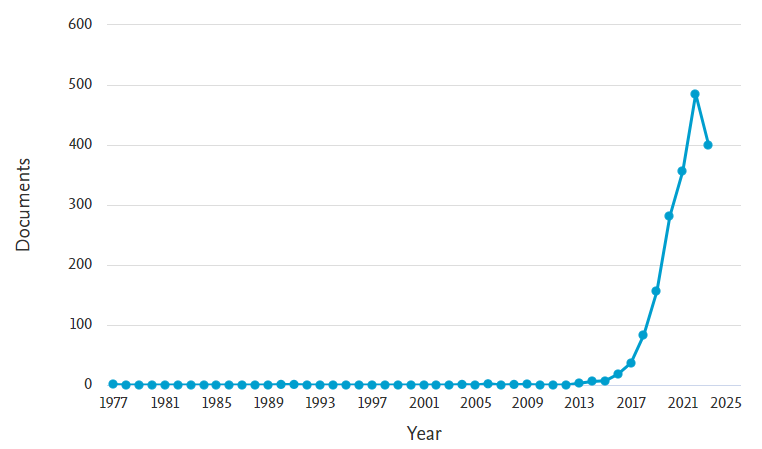
\includegraphics[width=0.8\linewidth]{Imagens/chap02/waam_papers.png}
    \caption{Contribuições de artigos publicados em jornais técnicos envolvendo WAAM. Fonte: SCOPUS.}
    \label{fig:waam_papers}
\end{figure}

Graças a grande quantidade de calor utilizada no processo, é comum que as peças produzidas sofram deformações e acumulem tensões residuais, levando ao risco de falhas. Além disso, baixa precisão geométrica e acabamento ruim são outros problemas causados pelo empilhamento de camadas de cordões \cite{ding2015wire}. A figura \ref{fig:waam_parts} mostra exemplos de peças produzidas por WAAM.

\begin{figure}[hbt!]
    \centering
    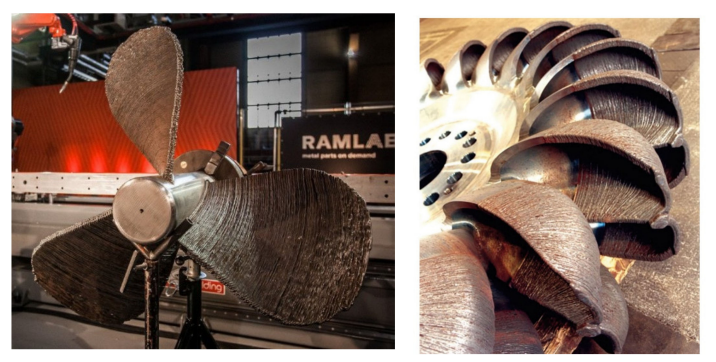
\includegraphics[width=0.8\linewidth]{Imagens/chap02/waam_parts.png}
    \caption{Hélice (esquerda) e tubina hídrica (direita) fabricados por WAAM \cite{feldmann20193d}.}
    \label{fig:waam_parts}
\end{figure}

\newpage
\subsection{Diferentes processos dentro da WAAM}
O processo de WAAM funciona através do depósito, camada a camada, do material metálico fundido pelo arco elétrico, que pode possuir diferentes fontes de energia. Os mais comuns são soldagem de arco de metal a gás (GMAW), soldagem de arco de metal Tungstênio a gás (GTAW) e soldagem a arco de plasma (PAW). \cite{pan2018arc}

\subsubsection{GMAW}
GMAW é um processo de soldagem no qual um arco elétrico se forma entre um eletrodo de arame metálico (que se consome no processo) e a base de trabalho. O arame geralmente está perpendicular ao plano da base. Existem diferentes métodos de extrusão do arame dentro do processo de GMAW, como por exemplo pulso-spray, spray ou transferência de metal a frio (CMT), uma variante do padrão de GMAW onde o arame é retraído e extrudado periodicamente com o intuito de controlar a transferência das gotículas de metal fundido. Esse método é o mais utilizado pela pequena quantidade de calor necessária \cite{pan2018arc}. A figura \ref{fig:gmaw_scheme} ilustra o processo de GMAW.

\begin{figure}[hbt!]
    \centering
    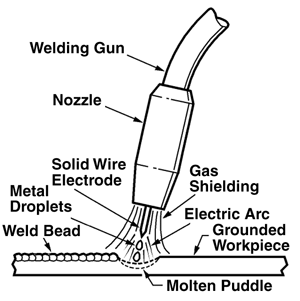
\includegraphics[width=0.6\linewidth]{Imagens/chap02/gmaw_scheme.png}
    \caption{Ilustração do processo de GMAW \cite{azadi2017simultaneous}.}
    \label{fig:gmaw_scheme}
\end{figure}

\subsubsection{GTAW}
No processo de GTAW, um eletrodo de tungstênio, não consumido, é usado para fundir um outro arame metálico, cujo material é depositado, como ilustrado na figura \ref{fig:gtaw_scheme}. Durante o processo de deposição, a orientação da alimentação do arame influencia a qualidade da transferência. Um modelo matemático foi desenvolvido para otimizar a direção e posição da alimentação do arame para melhorar a acurácia da deposição \cite{geng2017optimization}.

\begin{figure}[hbt!]
    \centering
    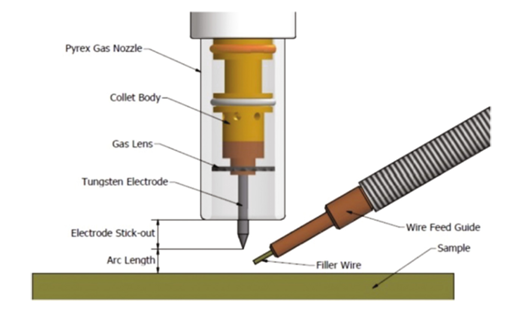
\includegraphics[width=0.8\linewidth]{Imagens/chap02/gtaw_scheme.png}
    \caption{Ilustração do processo de GTAW \cite{hoye2015characterisation}.}
    \label{fig:gtaw_scheme}
\end{figure}

\subsubsection{PAW}
O processo de PAW consiste num arco de plasma cuja densidade energética pode chegar a 3 vezes maior que o mesmo via GTAW, causando menos distorção nas soldas e menores pontos de solda, bem como maiores velocidades de soldagem, como ilustrado na figura \ref{fig:paw_scheme}. 

\begin{figure}[hbt!]
    \centering
    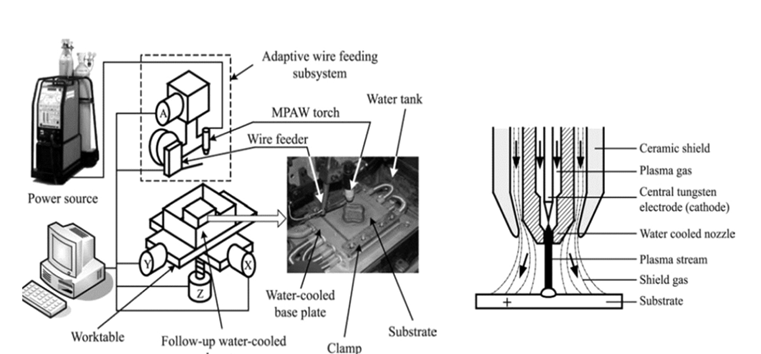
\includegraphics[width=0.7\linewidth]{Imagens/chap02/paw_scheme.png}
    \caption{Ilustração do processo de PAW e detalhes do arco de plasma \cite{aiyiti2006investigation}.}
    \label{fig:paw_scheme}
\end{figure}

\newpage
A figura \ref{fig:waam_steps} mostra as etapas da produção de uma peça via WAAM. São elas:
\begin{enumerate}[label=(\textit{\roman*})]
    \item Projeto da peça em software CAD, e adaptações necessárias para conformar-se ao processo de WAAM.
    \item  Definição da altura da camada e fatiamento em software dedicado.
    \item Definir a trajetória do maçarico, controlado por um manipulador robótico.
    \item Especificar a geometria do cordão durante a impressão.
    \item Definir os parâmetros de deposição indireta (IDP) para alcançar as características desejadas.
    \item Configurar os parâmetros de deposição na fonte de energia e mandar a trajetória para o robô. 
    \item Construir a peça. 
    \item Executar o pós-processamento da peça, atingindo o acabamento ou acurácia geométrica desejados.
\end{enumerate}

\begin{figure}[hbt!]
    \centering
    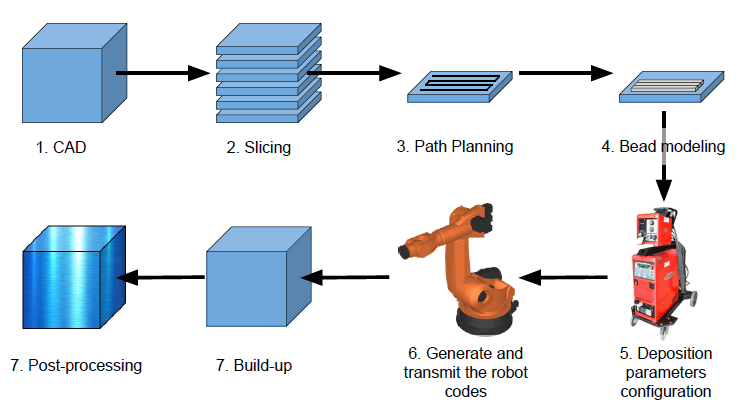
\includegraphics[width=0.8\linewidth]{Imagens/chap02/waam_steps.png}
    \caption{Etapas do processo de WAAM \cite{ding2016bead}.}
    \label{fig:waam_steps}
\end{figure}

\subsection{Defeitos comuns na WAAM}
Para que os sistemas de WAAM sejam amplamente utilizados na indústria, é necessário investigar e mitigar os defeitos de fabricação dessa tecnologia. Porosidade, deformação, tensão residual e craqueamento são alguns desss defeitos, que precisam ser evitados a fim de que as peças possam ser utilizadas em sua plena capacidade. Esses defeitos podem acontecer por conta de trajetórias não otimizadas durante a fabricação, configuração errada dos parâmetros de deposição, deformação associada ao acúmulo de calor, arames de baixa qualidade, contaminação, etc \cite{wu2018review}. A figura \ref{fig:waam_defects} descreve as correlações entre possíveis defeitos na fabricação via WAAM utilizando aço. 

\begin{figure}[hbt!]
    \centering
    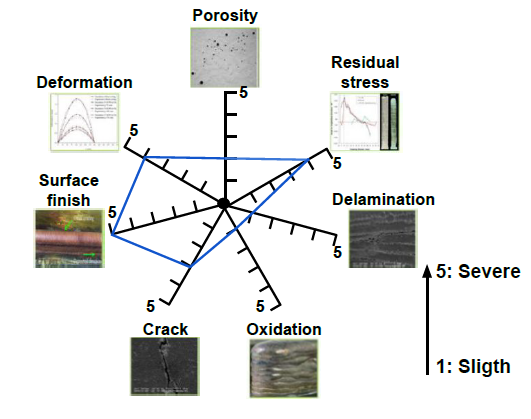
\includegraphics[width=0.8\linewidth]{Imagens/chap02/waam_defects.png}
    \caption{Correlação entre defeitos de fabricação via WAAM utilizando aço. Adaptado de \cite{wu2018review}.}
    \label{fig:waam_defects}
\end{figure}

\subsubsection{Tensão residual}
A tensão residual é o principal agente causador das distorções, que podem levar a falhas mecânicas. Ela consiste nas tensões internas que permanecem após todas as forças internas serem removidas, e é causada principalmente pela expansão e encolhimento causado pelo rápido aquecimento e esfriamento da peça. É impossível eliminá-la completamente, visto que o processo de WAAM depende de grandes quantidades de calor, no entanto, é possível mitigá-la com o tratamento térmico após a fabricação \cite{wu2018review}. 

\subsubsection{Porosidade}
Outro defeito comum presente no processo de WAAM é a presença de poros nas peças. Essa porosidade é causada por diversos fatores, como contaminação do arame, acúmulo de gases na peça, trajetórias não otimizadas, etc. Para reduzir este defeito, é necessário evitar os problemas descritos acima \cite{wu2018review}. 

\subsubsection{Delaminação}
A delaminação consiste na separação das camadas de impressão via WAAM. Ela acontece principalmente quando não há a fusão completa das camadas adjacentes, podendo ser visível por inspeção visual. Pré aquecer o substrato pode previnir este defeito \cite{wu2018review}.

\subsection{Parâmetros diretos e indiretos de deposição}
Os parâmetros de deposição podem ser divididos entre diretos (DDP) e indiretos (IDP) \cite{ozcelik2003modeling}. Os DDP são os parâmeteos de "saída", e estão relacionados com as características do material depositado, como geometria do cordão, propriedades mecânicas, etc. Já os IDP são os parâmetros de "entrada", e são as configurações utilizadas para se alcançar uma determinada característica desejada, como corrente (I), tensão (V), velocidade de viagem (TS), velocidade de alimentação do arame (WFS), entre outros. A figura \ref{fig:waam_params} descreve ambos os grupos de parâmetros. 

\begin{figure}[hbt!]
    \centering
    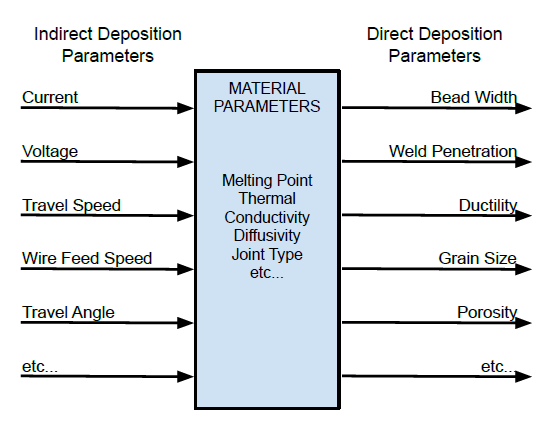
\includegraphics[width=0.8\linewidth]{Imagens/chap02/waam_params.png}
    \caption{Parâmetros de entrada e saída. \cite{ozcelik2003modeling}.}
    \label{fig:waam_params}
\end{figure}

\subsubsection{Corrente}
A corrente é um IDP elétrico intrínseco a fonte utilizada na soldagem via WAAM. Mantendo todos os outos parâmetros fixos, a corrente (I) influencia diretamente a velocidade de alimentação do arame (WFS) modelada na equação \ref{eq:current_wfs}

\begin{equation}
WFS = aI + bl_{so}I^2
\label{eq:current_wfs}
\end{equation}

onde $a$ é a constante de proporcionalidade para o aquecimento do anodo/catodo, cuja magnitude depende da polaridade, composição e outros fatores; $b$ é outra constante de proporcionalidade relacionada a resistência térmica, e $l_{so}$ é a extensão máxima (\textit{stick-out}) do eletrodo. Além disso, o aumento da corrente resulta em:

\begin{enumerate}
    \item Maior taxa de deposição (DR).
    \item Maior profundidade e largura de penetração do cordão.
    \item Maior largura e altura do cordão.
\end{enumerate}

\subsubsection{Tensão}
A tensão é um IDP importante no processo de GMAW, influenciando na própria corrente mencionada acima, no comprimento do arco, e outros IDPs.

\subsubsection{Velocidade de viagem do maçarico}
A velocidade de viagem (TS) é um parâmetro de deposição que depende da trajetória do robô, determinada pelo processo de deposição. A TS é simplesmente o módulo da velocidade linear tangente a curva da trajetória do robô, como mostrado na equação \ref{eq:ts_eq}. 

\begin{equation}
TS = \sqrt{V_x^2 + V_y^2}
\label{eq:ts_eq}
\end{equation}

A TS influencia as características do cordão e por isso é um importante IDP, sendo desejado que seja mantida constante durante a impressão para evitar variações na geometria do cordão. A TS também influencia outros DDPs, por exemplo, na penetração e largura do cordão. Quanto maior for a TS, menor são esses parâmetros mencionados \cite{ozcelik2003modeling}.

\subsubsection{Velocidade de alimentação do arame}
A velocidade de alimentação do arame (WFS) consiste na velocidade em que o arame é extrudado do local onde está armazenado em direção ao maçarico, onde será fundido e depositado. A WFS influencia positivamente a altura do cordão soldado. \cite{srivastava2023wire}.

% Além da TS, a distância entre o tubo e a base de trabalho e o fluxo de gás de proteção são alguns dos IDP definidos na etapa de planejamento e executadas durante a deposição. Em GMAW o gás de proteção serve para canalizar o arco elétrico. 

A figura \ref{fig:gmaw_idp_ddp} descrevem os IDP e DDP dentro do processo de GMAW.
\begin{figure}[hbt!]
    \centering
    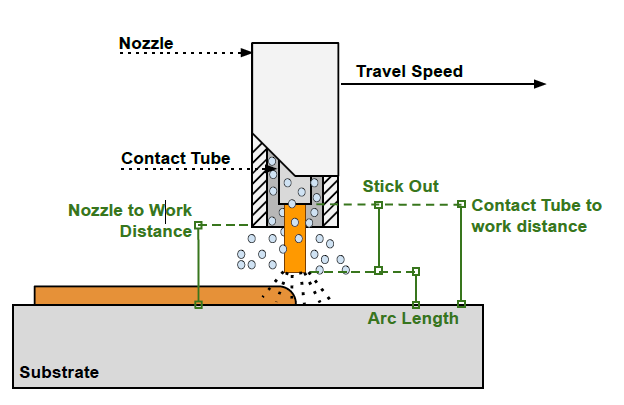
\includegraphics[width=0.46\linewidth]{Imagens/chap02/gmaw_idp.png}
    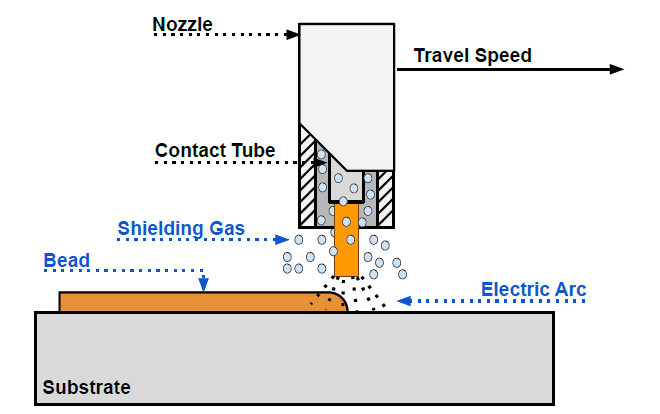
\includegraphics[width=0.46\linewidth]{Imagens/chap02/gmaw_ddp.png}
    \caption{Alguns IDPs (esquerda) en DDPs (direita) do processo de GMAW \cite{ozcelik2003modeling}.}
    \label{fig:gmaw_idp_ddp}
\end{figure}

% \begin{figure}[hbt!]
%     \centering
%     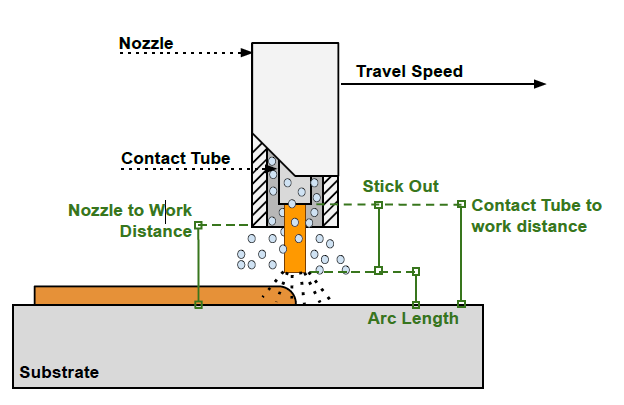
\includegraphics[width=0.8\linewidth]{Imagens/chap02/gmaw_idp.png}
%     \caption{TS e outros IDPs do processo GMAW \cite{ozcelik2003modeling}.}
%     \label{fig:gmaw_idp}
% \end{figure}

% \begin{figure}[hbt!]
%     \centering
%     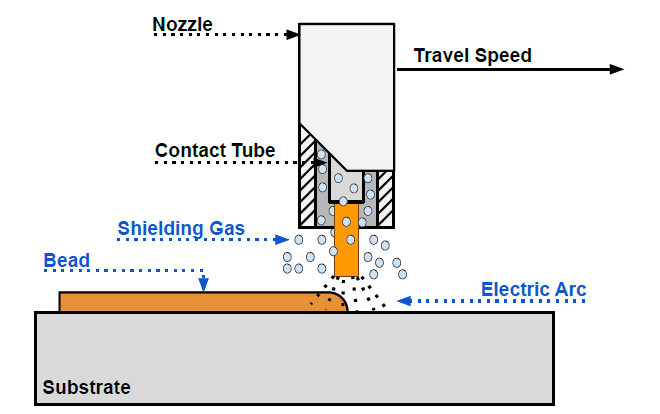
\includegraphics[width=0.8\linewidth]{Imagens/chap02/gmaw_ddp.png}
%     \caption{Visão lateral do maçarico no processo GMAW e alguns DDPs \cite{ozcelik2003modeling}.}
%     \label{fig:gmaw_ddp}
% \end{figure}

\newpage
\subsection{Geometria do cordão simples}
Como descrito anteriormente, é de suma importância entender as relações entre os parâmetros de deposição e a geometria do cordão simples. Alguns métodos matemáticos foram desenvolvidos para representar o perfil geométrico do cordão, correlacionando-o com os parâmetros de entrada (alguns mais simples, como parábolas, arcos circulares, e outros mais complexos, funções logísticas ou gaussianas). De forma geral, o principal parâmetro que influencia na geometria do cordão é a velocidade de alimentação do arame (WFS) e a velocidade de viagem (TS) \cite{cao2011overlapping}. 

Possuir um modelo geométrico robusto é de suma importância para o desenvolvimento de um sistema de MA inteligente e moderno, já que pode ser utilizado em uma malha de controle realimentado, aumentando a qualidade do acabamento das peças fabricadas via WAAM. 

Neste trabalho será utilizado apenas modelos de cordão simples no processo de GMAW. A próxima seção aborda toda a modelagem do simulador utilizado para gerar os dados que alimentam a rede.

\section{Simulação geométrica em GMAW}
\label{sec:simulation}
Diversos modelos estáticos de equações de transferência de massa e energia foram desenvolvidos ao longo dos anos para analisar as dinâmicas do processo de WAAM. Neste trabalho, será utilizado uma simulação para um modelo de cordão simples impresso em GMAW como fonte de geração de dados para o treinamento da rede. 

A modelagem em questão relaciona os parâmetros de entrada $f$ (WFS), $I_r$ (corrente), $l_c$ (Distância entre a ponta do arame e a base - CTWD) e $v$ (TS), e os parâmetros de saída $w$ (largura) e $h$ (altura) do cordão único. Essa modelagem acontece em duas etapas: a primeira consiste no processo GMAW, que relaciona os quatro parâmetros de entrada aos parâmetros $Q$ (potência líquida) e $A_c$ (área de seção reta), e a segunda consiste num modelo geométrico estático que relaciona esses dois parâmetros com a largura e altura do cordão, como ilustra a figura \ref{fig:sim_blocks}

\begin{figure}[hbt!]
    \centering
    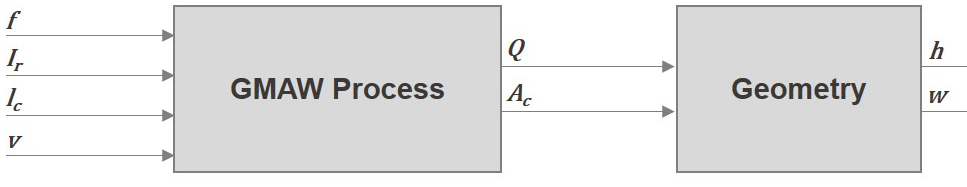
\includegraphics[width=0.8\linewidth]{Imagens/chap02/sim_blocks.png}
    \caption{Diagrama de blocos da modelagem utilizada \cite{bendia2021multivariable}.}
    \label{fig:sim_blocks}
\end{figure}

\subsubsection{Modelo do processo GMAW}
O modelo do processo GMAW consiste num modelo não linear de 5ª ordem (figura \ref{fig:gmaw_model}) considerando a dinâmica elétrica da fonte e a dinâmica térmica da deposição da gotícula metálica do cordão. 

\begin{figure}[hbt!]
    \centering
    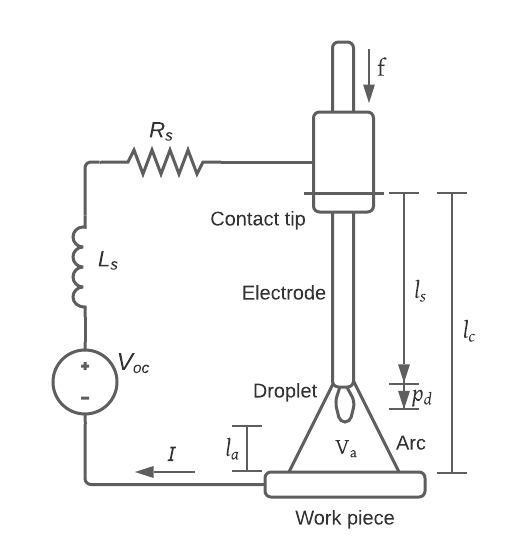
\includegraphics[width=0.5\linewidth]{Imagens/chap02/gmaw_model.png}
    \caption{Modelo termoelétrico do processo GMAW \cite{bendia2021multivariable}.}
    \label{fig:gmaw_model}
\end{figure}

A dinâmica elétrica da fonte que modela a transferência de energia é dada pela equação:

\begin{equation}
    \frac{dI}{dt} = \frac{1}{L_s} [V_{oc} - (R_a+R_s+R_L)I - V_0 -E_a(l_c-l_s)]
\end{equation}

onde $L_s$ é a indutância da fonte, $V_{oc}$ é a tensão de circuito aberto da fonte, $R_s$ é a resistência da fonte, $R_a$ é a resistência do arco, $R_L$ é an resistência do eletrodo, $V_0$ é a constante da zona de carga, $E_a$ é o fator de comprimento do arco e $l_s$ é a extensão do arame.  A resistência do eletrodo $R_L$ é função do comprimento: 
\begin{equation}
    R_L = \rho[l_s + 0.5(r_d+p_d)]
\end{equation}
onde $\rho$ é a resistividade do eletrodo, $r_d$ é o raio da gotícula e $p_d$ é a distância entre o centro de massa da gotícula e o eletrodo \cite{bendia2021multivariable}. Considerando uma fonte onde a corrente de deposição $I$ é mantida controlada numa corrente de referência $I_r$, $V_{oc}$ é usada como uma variável de controle definida por: 

\begin{equation}
    V_{oc} = K_v(I_r-I) + \bar{V}_{oc}
\end{equation}

onde $\bar{V}_{oc}$ é o ponto de opperação da tensão de circuito aberto e $K_v$ é um ganho proporcional. Portanto, a dinâmica da corrente em malha fechada é:

\begin{equation}
    \frac{dI}{dt} = \frac{1}{L_s} [K_vI_r - (R_a+R_s+\rho l_S + K_v)I + \bar{V}_{oc} - V_0 -E_a(l_c-l_s)]
\end{equation}

A tensão $V_a$ e potência $P_a$ do arco são:
\begin{align}
    V_a = V_0 + R_aI + E_a(l_c-l_s) \\
    P_a =  R_aI^2 + [E_a(l_c-l_s) + V_0]I
\end{align}

Finalmente, a taxa de transferência de energia do arco para a base é modelada pela eficiência $\eta$, e a potência líquida $Q$ é:
\begin{equation}
    Q = \eta P_a
\end{equation}

A equação de balanço de massa é definida como a diferença entre o material entrando no sistema, que depende da WFS $f$, e o material saindo o sistema, através da deposição da solda. Assumindo que a densidade do eletrodo $\rho_w$ é constante, o fluxo de material que entra é definido como $A_w f$, onde $A_w$ é a área de seção reta do arame. Já o fluxo de material que sai é definido como $M_r$. Com isso, a dinâmica do balanço de massa é:
\begin{align}
    A_w\frac{dl_s}{dt} &= Aw f - M_r \\
    M_r &= C_2\rho l_s I^2 + C_1 I
\end{align}
onde $C_1$ e $C_2$ são constantes de fusão.

Da perspectiva de um sistema de coordenadas movendo-se junto com o maçarico com velocidade $v$, como mostrado na figura \ref{fig:torch_coords}, o fluxo volumétrico de deposição do cordão é definido como $\frac{dV}{dt} = A_c v$. O volume depositado é igual ao fluxo de saída do material $M_r$. Portanto, $M_r = A_c v$:
\begin{equation}
    A_c = \frac{C_2\rho l_s I^2 + C_1 I}{v}
\end{equation}

\begin{figure}[hbt!]
    \centering
    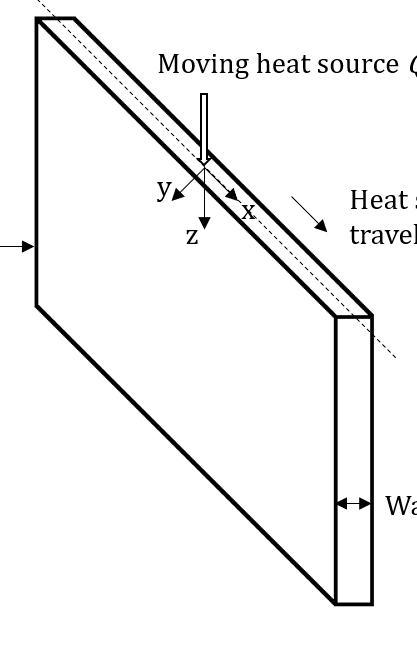
\includegraphics[width=0.2\linewidth]{Imagens/chap02/torch_coords.png}
    \caption{Sistemas de coordenadas do maçarico \cite{bendia2021multivariable}.}
    \label{fig:torch_coords}
\end{figure}

Com isso, a dinâmica do processo é definida pelo sistema não linear \cite{bendia2021multivariable}:
\begin{align}
    \frac{dl_s}{dt} &=-\frac{1}{A_w}(C_2\rho l_s I^2 + C_1 I) + f \\
    \frac{dI}{dt} &= \frac{1}{L_s} [K_vI_r - (R_a+R_s+\rho l_S + K_v)I + \Delta V_0 -E_a(l_c-l_s)]
\end{align}

onde $\Delta V_0 = \bar{V}_{oc} - V_0$. As variáveis de estado são $l_s (m)$ e $I (A)$, os parâmetros de entrada são $f (m/s)$ e $I_r (A)$, e os de saída são $Q (W)$ e $A_c (m^2)$. 

\subsubsection{Modelo geométrico}
As dimensões do cordão podem ser calculadas do campo de temperaturas no substrato no entorno de uma fonte de calor em movimento (o maçarico). A curva isotérmica correspondente a temperatura de fusão dá a forma da piscina de fusão. Considerando uma parede fina de substrato como mostrado na figura \ref{fig:torch_coords}, a solução de Rosenthal é:

\begin{equation}
    T - T_0 = \frac{Q}{2\pi k w_t}K_0\left(\frac{r_{xz}v}{2\alpha}\right)\exp{\frac{-xv}{2\alpha}} \label{eq:rosenthal}
\end{equation}

onde $T$ é a temperatura de um ponto nas coordenadas $(x,z)$ em relação ao maçarico, $T_0$ é a temperatura do substrato na saída do maçarico, $k$ é a condutividade térmica, $\alpha$ é a difusividade térmica, $w_t$ é a espessura da parede, $v$ é a TS, $r_{xz} = \sqrt{x^2+z^2}$ é a distância euclidiana do ponto ao maçarico e $K_0$ é a função de Bessel modificada de ordem zero do segundo tipo. Em \cite{rios2018analytical} uma extensão de \ref{eq:rosenthal} é proposta para calcular a potência desejada a fim de alcançar uma determinada dimensão geométrica:

\begin{equation} 
    Q = 4kw_e(T_m-T_0)(0.2+\frac{v}{2\alpha}d_a) \label{eq:rios}
\end{equation}

onde $T_m$ é a temperatura de fusão, $w_e$ é a largura efetiva do cordão e $d_a$ é a profundidade aparente do cordão. As características geométricas do cordão estão ilustradas na figura \ref{fig:bead_geom} e são calculadas por:
\begin{align}
    w &= 2r \label{eq:w}\\
    w_e &= 2ra\cos(\theta/2) \\
    h &= 2r\sin(\theta/2) \\
    d_a &= \frac{w+h}{2} \label{eq:d_a} \\
\end{align}

\begin{figure}[hbt!]
    \centering
    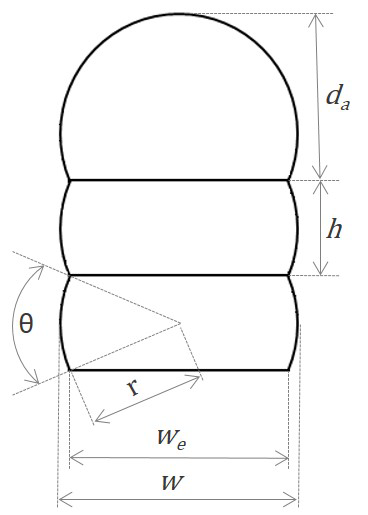
\includegraphics[width=0.3\linewidth]{Imagens/chap02/bead_geom.png}
    \caption{Parâmetros geométricos do cordão \cite{bendia2021multivariable}.}
    \label{fig:bead_geom}
\end{figure}

A área da camada única do cordão $A_c$ é dada por:
\begin{equation}
    A_c = 0.5(w^2\arctan(h/w_e) + w_eh)
\end{equation}
Para  $h < \frac{w_e}{2} < \frac{w}{2}$, então $\frac{h}{w_e} < \frac{1}{2}$ e $\arctan(h/w_e) \approx h / w_e$, então:
\begin{equation}
    A_c = \frac{1}{2} \left(w^2\frac{h}{w_e} + w_e h\right) \label{eq:area_bead}
\end{equation}
Considerando a área útil dada pelo produto $w_e h$ então a eficiência de deposição é:
\begin{equation}
    \eta_d = \frac{w_e h}{A_c} \label{eq:eta_d}
\end{equation}

Substituindo \ref{eq:area_bead} in \ref{eq:eta_d} para achar a relação entre $w$ e $w_e$:
\begin{equation}
    w = \sqrt{\frac{2-\eta_d}{\eta_d}}w_e
\end{equation}

Com isso, considerando as equações \ref{eq:w}-\ref{eq:d_a} e \ref{eq:area_bead} em \ref{eq:rios}, $w_e$ pode ser expresso em função de $Q$, $v$ e $A_c$:
\begin{equation}
    \sqrt{(2-\eta_d)/eta_d}w_e^2 + 0.8\frac{\alpha}{v}w_e + \eta_dA_c - \frac{Q\alpha}{k\Delta T v} = 0
\end{equation}

onde $\Delta T = T_m - T_0$. Esse polinômio do segundo grau tem raízes se $p = \left(\eta_d-\frac{Q\alpha}{k\Delta T v}\right)/\sqrt{\frac{2-\eta_d}{\eta_d}}$ for negativo. Essa condição é satisfeita se:
\begin{equation}
    Q > \frac{k\Delta T v}{\alpha} \eta_d A_c \label{eq:q_cond}
\end{equation}
 
Portanto, se \ref{eq:q_cond} for satisfeita, $w_e$ e $h$ são dados por:
\begin{align}
    w_e &= -\frac{0.4\alpha}{k_w v} + \sqrt{\left(\frac{0.4\alpha}{k_wv}\right)^2 - \frac{1}{k_w}\left(\frac{2A_c}{k_w^2+1} - \frac{Q\alpha}{k\Delta T v}\right)} \\
    h &= \eta_d \frac{A_c}{w_e}
\end{align}

onde $k_w = \sqrt{(2-\eta_d)/\eta_d}$.

% \subsubsection{Linearização do modelo}

\section{\textit{Machine Learning}}
\textit{Machine Learning} (ML), ou aprendizado de máquinas, são algoritmos e processos em que a máquina não sabe a resposta para determinada tarefa. No caso deste projeto, focamos nos algoritmos de ML para análise de dados. Esses algoritmos podem ser de aprendizado supervisionado ou não-supervisionado. Porém, tão importante quanto saber qual o melhor algoritmo utilizar, é saber quais dados utilizar, bem como processá-los \cite{alpaydin2020introduction}. A base de treinamento dos modelos de ML são os dados. É de suma importância possuir dados de qualidade, que tenham riqueza da informação que é necessária para aquele determinado problema. 

\subsection{Métodos de aprendizado}
O aprendizado de todos os modelos e algoritmos de ML pertencem a um desses três grupos: Aprendizado Supervisionado, Não supervisionado, ou por reforço.  No caso do aprendizado supervisionado, os dados de entrada $X$ e saída $Y$ são conhecidos. Com isso, a tarefa consiste em utilizar $X$ para produzir uma estimativa $\hat{Y}$ que é comparada a $Y$. No aprendizado não supervisionado, os dados de saída $Y$ não são conhecidos, e a tarefa é estimar os valores de saída de cada ponto de $X$ de forma que pontos distintos possuem valores de $y$ distintos, e pontos próximos possuem valores de $y$ próximos. Por último, os algoritmos de aprendizado por reforço funcionam com a recompensa positiva ou negativa de determinadas ações, que são usadas para treinar uma política que consegue escolher aquela ação que maximiza a recompensa. 

\subsection{\textit{Deep Learning}}
A área do \textit{Deep Learning} (DL) consiste na modelagem das redes neurais artificiais (ANN), que se inspiram no cérebro humano. A primeira e mais básica dela é o Perceptron Multicamadas (MLP), que utiliza uma rede de neurônios interconectados que realizam operações matemáticas a fim de mapear, via aprendizado supervisionado, dados de entrada $X$ e de saída $Y$. 

\subsubsection{MLP}
O neurônio funciona recebendo um vetor de valores de entrada $\mathbf{x}$ nos seus dendritos, produzindo uma saída $z = \mathbf{w}^T\mathbf{x} + b$, onde $\mathbf{w}$ é o vetor de pesos para cada braço do dendrito e $b$ é o viés do neurônio. A saída $z$ então é usada como entrada em uma função de ativação $\phi(z)$ que produz uma ativação $\alpha$, que se assemelha ao potencial de ativação do neurônio humano. Essa ativação então é passada adiante pelo axônio para os dendritos dos neurônios nas camadas posteriores. A rede de neurônios consiste em camadas de neurônios: a primeira camada é chamada  camada de entrada, que recebe os dados de entrada $X$, a última camada se chama camada de saída, que produz a estimativa $\hat{Y}$ que é comparada aos dados observados $Y$. A figura \ref{fig:mlp_scheme} ilustra o esquema de um neurônio (esquerda) e de uma rede neural (direita) com uma camada escondida \cite{alpaydin2020introduction}.

\begin{figure}[hbt!]
    \centering
    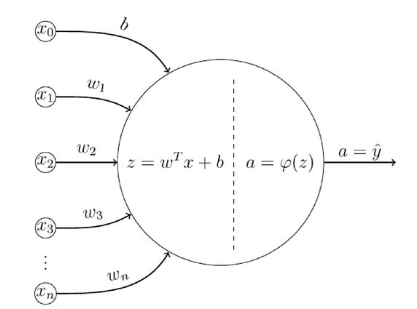
\includegraphics[width=0.46\linewidth]{Imagens/chap02/neuron_scheme.png}
    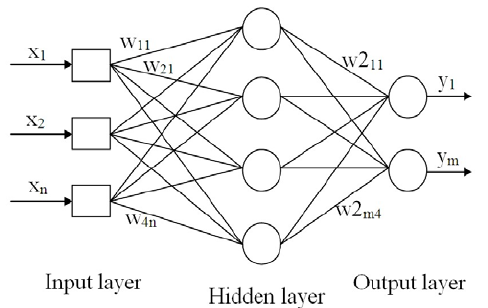
\includegraphics[width=0.46\linewidth]{Imagens/chap02/mlp_scheme.png}
    \caption{Esquema de neurônio (esquerda) e rede neural MLP (direita) \cite{minsky1969perceptrons}.}
    \label{fig:mlp_scheme}
\end{figure}

\subsubsection{Erros de estimação}
O treinamento da rede consiste, então, na minimização do erro entre $\hat{Y}$ e $Y$, que pode ser:
\begin{enumerate}
    \item Erro Absoluto Médio (MAE):
    \begin{equation}
        J_{MAE} = \frac{1}{m} \sum_{i=1}^m |y^{(i)} - \hat{y}^{(i)}|
    \end{equation}
    \item Erro Quadrático Médio (MSE):
    \begin{equation}
        J_{MSE} = \frac{1}{m} \sum_{i=1}^m (y^{(i)} - \hat{y}^{(i)})^2
    \end{equation}
    \item Entropia Cruzada: 
    \begin{equation}
        J_{CE} = -\frac{1}{m}[y^{(i)}\log(\hat{y}^{(i)}) + (1-y^{(i)})\log(1-\hat{y}^{(i)})]
    \end{equation}
\end{enumerate}

\subsubsection{\textit{Backpropagation}}
Este erro é utilizado para ajustar o vetor de pesos $\mathbf{w}$ e o viés $b$ da camada de saída através de otimizadores clássicos, e das demais camadas da rede neural através do algoritmo de \textit{backpropagation} \cite{hecht1992theory}, o cerne das redes neurais, que utiliza o ajuste de um neurônio para ajustar os neurônios conectados ao seus dendritos (entrada) conforme as equaçãões \ref{eq:backprop_start}-\ref{eq:backprop_end}:

\begin{align}
    \frac{\partial J}{\partial y_i} &= \frac{\partial J}{\partial o}\frac{\partial w}{\partial y_i} \label{eq:backprop_start}  \\
    y_i &= \phi(z) \\
    z &= \mathbf{w}^T\mathbf{x} + b \\
    \frac{\partial o}{\partial y_i} &= \frac{\partial o}{\partial z}\frac{\partial z}{\partial y_i}  = \frac{\partial o}{\partial z}w_i \label{eq:backprop_end}
\end{align}

onde $ \frac{\partial o}{\partial z}$ depende da função de ativação $\phi(z)$, $\frac{\partial J}{\partial o}$ é o ajuste conhecido do neurônio $o$, e $\frac{\partial J}{\partial y_i}$ é o ajuste estimado do neurônio $y_i$ conectado ao neurônio $o$ pelo peso $w_i$, como ilustrado na figura \ref{fig:backprop}.

\begin{figure}[hbt!]
    \centering
    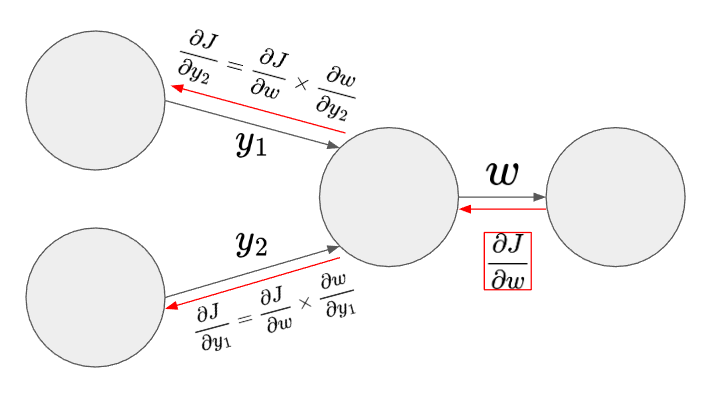
\includegraphics[width=0.8\linewidth]{Imagens/chap02/backprop.png}
    \caption{Ilustração do algoritmo de backpropagation. Fonte: o autor.}
    \label{fig:backprop}
\end{figure}

\subsubsection{Redes Neurais Convolucionais (CNN)}
As redes neurais convolucionais (CNN) são redes análogas às redes tradicionais como o MLP, no sentido de possuir um conjunto de neurônios que se otimizam a fim de aprender uma determinada tarefa. A diferença notável das redes convolucionais é a sua aplicação: para problemas que envolvem dados multidimensionais (tensores), como imagens, onde regiões próximas contém informações semelhantes, é recomendado o uso de CNNs. Isso porque ela permite a extração das características dessas imagens, que então alimentam uma rede MLP tradicional \cite{o2015introduction}, como ilustrado na figura \ref{fig:cnn_scheme}.

\begin{figure}[hbt!]
    \centering
    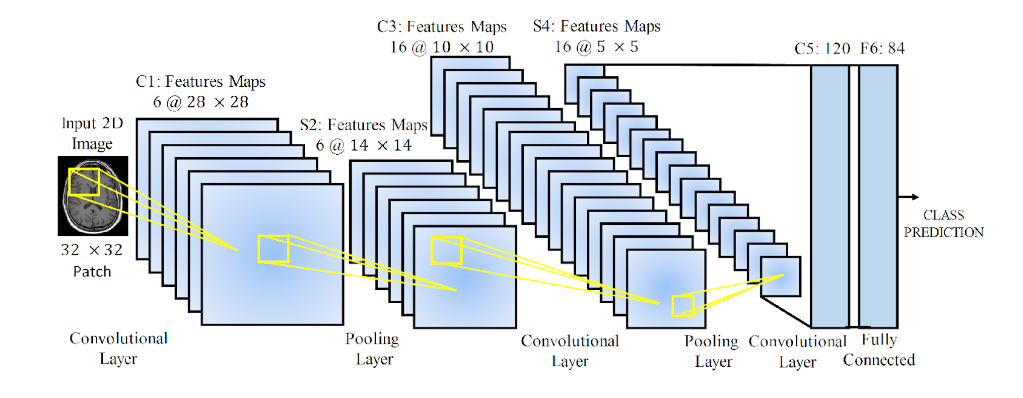
\includegraphics[width=0.8\linewidth]{Imagens/chap02/cnn_scheme.png}
    \caption{Esquema de uma CNN usada para análise de imagens de tomografia \cite{anwar2018medical}.}
    \label{fig:cnn_scheme}
\end{figure}

No caso das CNNs, em vez de valores únicos de pesos, cada conexão entre neurônios recebe uma matriz de pesos, chamados de filtros. Esses filtros então realizam uma operação de convolução com os dados recebidos (como ilustrado na figura \ref{fig:conv_scheme}), daí o nome da rede.

\begin{figure}[hbt!]
    \centering
    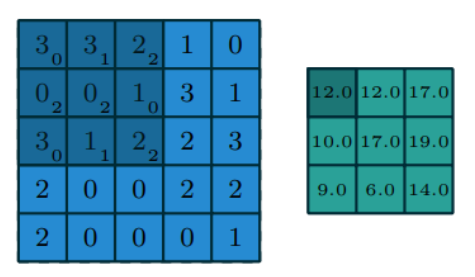
\includegraphics[width=0.5\linewidth]{Imagens/chap02/conv_scheme.png}
    \caption{Convolução entre o filtro (azule escuro) e os dados (azul claro). O resultado da convolução é a saída do neurônio (verde) \cite{odena2016deconvolution}.}
    \label{fig:conv_scheme}
\end{figure}

\subsubsection{Redes Neurais Recorrentes (RNN)}
As redes neurais recorrentes se destacam na solução de problemas que envolvem a identificação e modelagem de sistemas dinâmicos, utilizando dados de séries temporais. Por se tratar de dados que possuem algum interação estatística e temporal, a arquitetura das RNNs consiste numa cadeia de neurônios chamados células, que possuem um determinado estado oculto , que é definido como \cite{yu2019review}:
\begin{equation}
    y_t = h_t = \sigma(W_h h_{t-1}+W_xx_t+b)
\end{equation}

onde $h$ é o estado da célula, que depende do estado passado $h(t-1)$ pertencente a célula anterior, da entrada atual $x(t)$. $W_h$, $W_x$ são pesos e $b$ é um viés, todos os quais são parâmetros ajustados no treinamento.  A figura \ref{fig:rnn_cell} contém um esquema de uma célula de uma RNN.

\begin{figure}[hbt!]
    \centering
    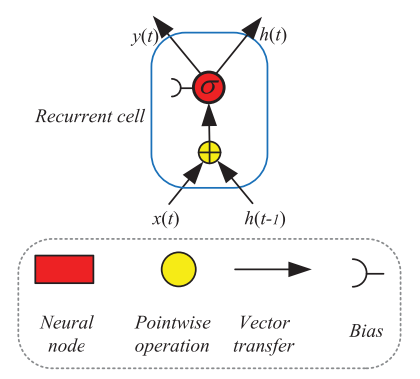
\includegraphics[width=0.5\linewidth]{Imagens/chap02/rnn_cell.png}
    \caption{Esquema de célula $\sigma$ recorrente padrão \cite{yu2019review}.}
    \label{fig:rnn_cell}
\end{figure}

Com o objetivo de lidar com problemas onde os dados das séries temporais possuem dependências estatísticas também a longo prazo, \cite{hochreiter1997long} propuseram a célula LSTM, que melhoraram a capacidade de memória da célula $sigma$ supracitada intoduzindo um "portão" dentro da célula. Este portão decide se a informação da entrada $x(t)$ vai ser jogada fora. O funcionamento da célula LSTM com portão de esquecimento ilustrada na figura \ref{fig:lstm_cell} é expresso como:
\begin{align}
    f_t &= \sigma(W_{fh}h_{t-1} + W_{fx}x_t + b_f) \\
    i_t &= \sigma(W_{ih}h_{t-1}+W_{ix}x_t+b_i) \\
    \Tilde{c}_t &= \tanh(W_{\Tilde{c}h}h_{t-1}+W_{\Tilde{c}x}x_t + b_{\Tilde{c}}) \\
    c_t &= f_t \cdot c_{t-1} + i_t \cdot \Tilde{c}_t \\   
    o_t &= \sigma(W_{oh}h_{t-1}+W_{ox}x_t+b_i) \\
    h_t &= o_t \cdot \tanh(c_t)
\end{align}

\begin{figure}[hbt!]
    \centering
    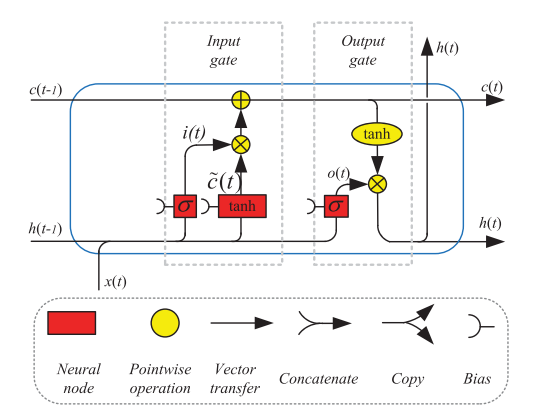
\includegraphics[width=0.6\linewidth]{Imagens/chap02/lstm_cell.png}
    \caption{Esquema de célula LSTM padrão \cite{yu2019review}.}
    \label{fig:lstm_cell}
\end{figure}

\newpage
\section{Controle MPC}
O Controle por Modelo Preditivo (MPC) é um método de controle eficiente e aplicado em diversos processos industriais. Ele consiste de três elementos básicos \cite{han2013nonlinear}:
\begin{enumerate}
    \item Modelo: Realiza a predição da evolução do sistema controlado, a partir da identificação da dinâmica do seu comportamento. Como o sistema modelado é não linear, o MPC desenvolvido é denominado NMPC. Pela complexidade da identificação desse sistema, surge a necessidade da utilização de redes neurais LSTM como a utilizada neste trabalho.
    \item Trajetória de referência: O comportamento alvo desjeado para as saídas do sistema, no caso a largura e altura do cordão.
    \item Otimizador: Estima o controle ótimo que minimiza uma determinada função custo estabelecida. Essa função geralmente possui duas parcelas: o erro de rastreamento e a regularização do sinal de controle.
\end{enumerate}

O comportamento preditivo do MPC permite, portanto, a previsão das saídas do sistema num determinado horizonte de tempo, possibilitando que ele não só rastreie uma determinada trajetória desejada como também minimize a função custo estabelecida. Ele é capaz de integrar controle ótimo, controle de processos, controle multivariável e referências futuras, simultâneamente \cite{han2013nonlinear}. A figura \ref{fig:mpc_scheme} ilustra a malha fechada de controle via NMPC.

\begin{figure}[hbt!]
    \centering
    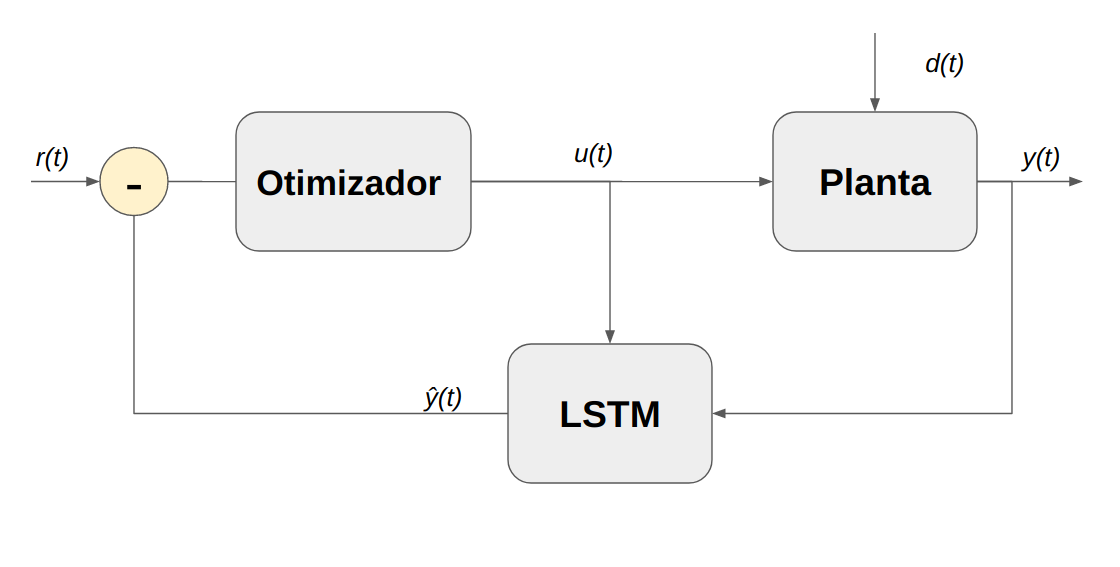
\includegraphics[width=0.7\linewidth]{Imagens/chap02/mpc_scheme.png}
    \caption{Esquema de malha fechada de controle via NMPC.}
    \label{fig:mpc_scheme}
\end{figure}

\subsection{Otimizador}
A otimização do controle NPMC em questão consiste na minimização de dois erros, o de rastreamento e de regularização, como no exemplo formulado abaixo:
\begin{align}
    \min_{U(t)} J(t) = \min_{U(t)} a \sum_{k=0}^{N-1}(r(t+k)&-y(t+k))^2 + b \sum_{k=0}^{M-1}u(t+k)^2 \\
    \text{sujeito a} \;\;\;\;& \\
    u_{min} \leq &u(t) \leq u_{max} \\
    y_{min} \leq &y(t) \leq y_{max}
\end{align}
onde $a$ e $b$ são pesos, $N$ o horizonte de predição da saída, $M$ o horizonte de predição de controle e $U(t)=[u(t), u(t+1), ..., u(t+M-1)]$ é o controle ótimo estimado. No instante $t$, calcula-se o controle $U(t)$ e utiliza como controle o primeiro ponto ($u^*(t) = U(t)$). Na seção \ref{sec:mpc_imp} será detalhada a otimização implementada neste trabalho.
% \chapter{Metodologia Proposta}
\label{chap3}
Todos os scripts desenvolvidos estão contidos no Apêndice \ref{appendice} e no diretório do  \href{https://github.com/lucascbarbosa/lstm-control-waam}{Github}.
\section{Geração dos dados}
\subsection{Simulação}
Os dados provenientes da simulação descrita na seção \ref{sec:simulation}, descrevem um sistema MIMO cujas entradas são a WFS $f$ e a corrente de referência da fonte $Ir$ e as saídas são a largura efetiva $w_e$ e a altura $h$ do cordão. Os valores das constantes utilizadas na simulação estão descritos na tabela \ref{tab:params_simulation} e são inicializados no script presente na seção \ref{code:gmaw_process}. Esses valores foram retirados de \cite{bendia2021multivariable}.

\begin{table}[hbt!]
    \centering
    \begin{tabular}{|c|c|}
    \hline
    Constante & Valor \\
    \hline
    $\eta$ & 0.655 \\
    \hline
    $\eta_d$ & 0.958 \\
    \hline
    $E_a$ & 723.2561 \\
    \hline
    $V_o$ & 5.1782 \\
    \hline
    $R_a$ & 0.0201 \\
    \hline
    $R_s$ & 0.004 \\
    \hline
    $L_s$ & 0.00014 \\
    \hline
    $V_{oc}$ & 31 \\
    \hline
    $k_v$ & 10 \\
    \hline
    $l_c$ & 0.01 \\
    \hline
    $v$ & 0.12 \\
    \hline
    $\Delta T$ & 1300 \\
    \hline
    $\rho$ & 0.1319 \\
    \hline
    $k$ & 24 \\
    \hline
    $\alpha$ & 7.79e-6 \\
    \hline
    $C_1$ & 3.2634e-10 \\
    \hline
    $C_2$ & 1.1836e-9 \\
    \hline
    $r_w$ & 0.0006 \\
    \hline
    $l_{so}$ & 0.0041 \\
    \hline
    $f_0$ & 0.055 \\
    \hline
    $Ir_0$ & 146 \\
    \hline
    $w_{e0}$ & 0.0041 \\
    \hline
    $h_0$ & 0.0012 \\
    \hline
    \end{tabular}
    \caption{Constantes utilizadas na simulação}
    \label{tab:params_simulation}
\end{table}

Os dados de entrada foram gerados utilizando sinais binários pseudoaleatórios com amplitude modulada (APRBS) \cite{deflorian2011design, miriyala2020deep}. Esses sinais consistem em degraus $u_k$ cujo período $T$ é constante e amplitude $A_k$ é uma variável aleatória discreta e uniforme cuja imagem $A$ de ordem $M$ é:
\begin{equation}
    A_k = u_{min} + (u_{max} - u_{min})i/(M-1)\; \;\;
    \forall i \in \{0, 1, 2, \ldots, M-1\}
\end{equation}
Onde $u_min$ e $u_max$ são as amplitudes mínima e máxima permitidas do degrau, respectivamente. A ordem M é definida como o número de pontos projetados. A tabela \ref{tab:params_aprbs} descreve os valores dos parâmetros $M$, $u_{min}$ e $u_{max}$ para os dados de treino e teste.

\begin{table}[hbt!]
    \centering
    \begin{tabular}{|c|c|c|c|c|c|c|}
    \hline
    Ensaio & $M$ & $N$ & $f_{min}$ & $f_{max}$ & $Ir_{min}$ & $Ir_{max}$ \\
    \hline
    Treino & 2 & 1000 & 0 & $f_0$ & 0.6$Ir_0$ & $Ir_0$ \\
    \hline
    Teste & 10 & 1000 & 0 & $f_0$ & 0.6$Ir_0$ & $Ir_0$  \\
    \hline
    \end{tabular}
    \caption{Parâmetros dos sinais APRBS gerados para a entrada da simulação.}
    \label{tab:params_aprbs}
\end{table}

O sinal $\mathcal{U}$ é, então, o trem de degraus:
\begin{align}
    \mathcal{U} &= \sum_{k=0}^{N}(A_k-A_{k-1}) u_k \\
    u_k &= u(t-kT)
\end{align}
onde N é o total de degraus do sinal. 
O \textit{script} encarregado de gerar esses dados está presente em \ref{code:generate_database}. As entradas são então utilizadas para produzir as saídas utilizando as equações da dinãmica do processo descritas na seção anterior. Além disso, foi adicionado um ruído gaussiano $\mathcal{N}(0,1)$.

\subsection{Dados experimentais}
Além dos dados de simulação, foram utilizados dados experimentais de impressão para validar o treinamento do modelo desenvolvido. Os dados se referem a um sistema SISO cuja entrada é a WFS $f$ e a saída é a largura efetiva do cordão $w_e$. Os testes experimentais foram conduzidos em \cite{novais2023adaptative} utilizando um sistema robótico composto por um braço robótico Kuka KR90 de 6DOF e uma mesa posicionadora Kuka KP2 de 2DOF, controlados por um controlador Kuka KRC4 com o complemento de software Kuka RSI.

\subsection{Tratamento dos dados}
O primeiro passo é a normalização dos dados. Os dados de entrada foram normalizados utilizando a normalização min-max (equação \ref{eq:minmax_norm}) enquanto os dados de saída foram normalizados utilizando a normalização média-variância (equação \ref{eq:meanvar_norm}).
\begin{equation}
    \label{eq:minmax_norm}
    y_{norm} = \frac{y-y_{min}}{y_{may}-y_{min}} 
\end{equation}
\begin{equation}
    \label{eq:meanvar_norm}
    y_{norm} = \frac{y-\mu_y}{\sigma_y} 
\end{equation}

Após isso, os dados de entrada e saída são sequenciados para gerar a base de dados utilizada para treinar a rede neural. A entrada $X$ da rede contém sequências pontos do passado da série temporal completa das entradas e saídas do sistem, enquanto a saída $Y$ contém os pontos das saídas um passo a frente. Assim, o objetivo da rede é, conhecendo uma sequência dos últimos $P$ pontos (de $k-P+1$ a $k$) das entradas $f$ e $I_r$ e dos últimos $Q$ pontos (de $k-Q+1$ a $k$) das saídas $w_e$ e $h$, estimar os valores de $w_e$ e $h$ $H$ passos a frente (instante $k+H$) \cite{miriyala2020deep}. O sequenciamento dos dados é descrito na figura \ref{fig:data_sequencing}:

\begin{figure}[hbt!]
    \centering
    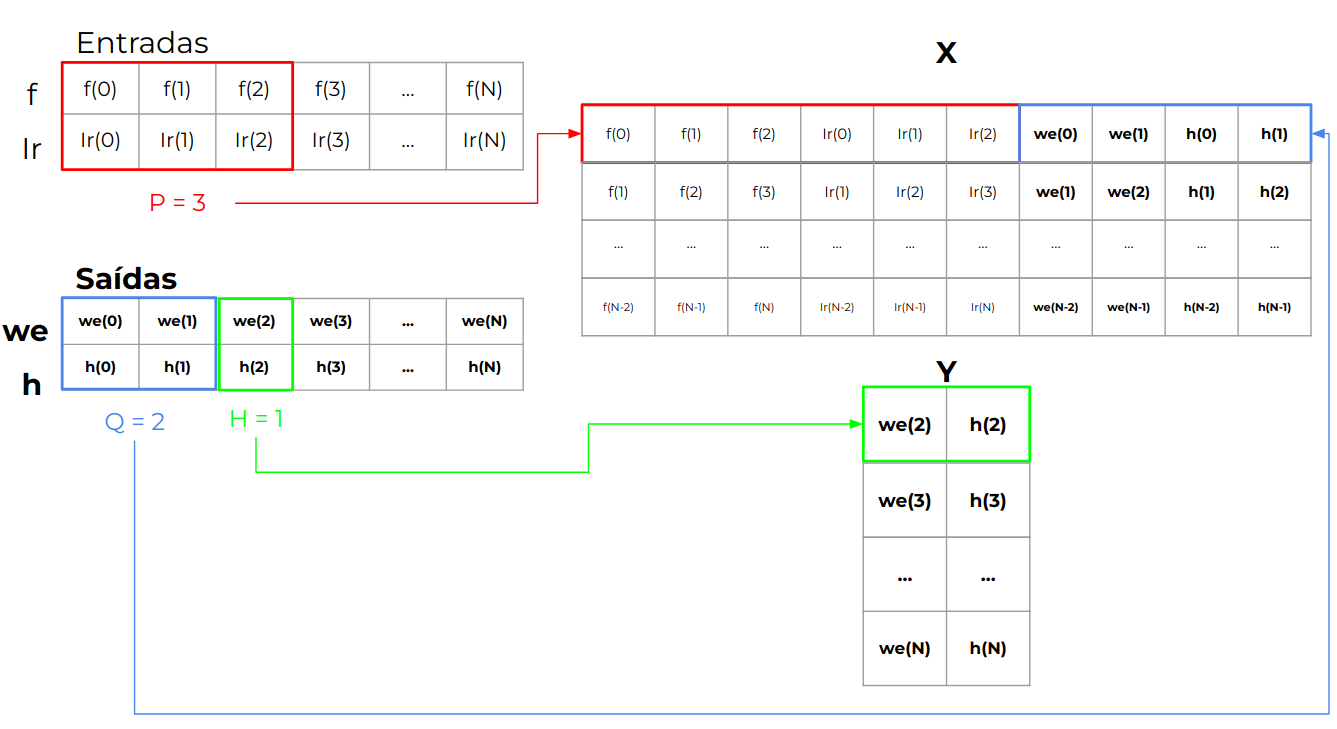
\includegraphics[width=\linewidth]{Imagens/chap03/data_sequencing.png}
    \caption{Sequenciamento dos dados gerados na simulação para $P=3$, $Q=2$ e $H=1$. Fonte: Autor.}
    \label{fig:data_sequencing}
\end{figure}

A influência dos parâmetros $P$, $Q$ e $H$ na performance da identificação da dinâmica serão analisados na seção de Resultados. O \textit{script} contendo as funções que realizam o processamento dos dados está presente em \ref{code:process_data}

\section{Definição da Rede}
\subsection{Arquitetura}
A rede neural neste trabalho foi desenvolvida utilizando o framework \textit{Keras/Tensorflow} em \textit{Python} \cite{tensorflow2015}. Ela consiste em duas camadas:
\begin{enumerate}
    \item Camada LSTM: Nesta camada, foram utilizados 64 células LSTM como a ilustrada na figura \ref{fig:lstm_cell}. A função de ativação utilizada foi a ReLU (Rectified Linear Unit), cuja equação é $f(x) = \max(0,x)$.
    \item Camada MLP: Nesta camada, foram utilizados 2 neurônios clássicos como o ilustrado na figura \ref{fig:mlp_scheme}, com a mesma função de ativação ReLU. A função desta camada é reduzir a dimensão da saída para a mesma das amostras de $Y$, no caso um vetor de 2 elementos ($w_e$ e $h$).
\end{enumerate}
A função de custo utilizada é o MSE, por se tratar de um problema de regressão, e o otimizador utilizado é o Adam \cite{kingma2014adam}, o estado da arte de otimizadores na área de \textit{Deep Learning}, por ser computacionalmente eficiente, ter pouco requisito de memória, ser invariante ao reescalonamento diagonal de gradientes e ser adequado para problemas grandes em termos de dados/parâmetros. A figura \ref{fig:model_summary} ilustra o diagrama de blocos da rede, com as especificações de cada camada.

\begin{figure}[hbt!]
    \centering
    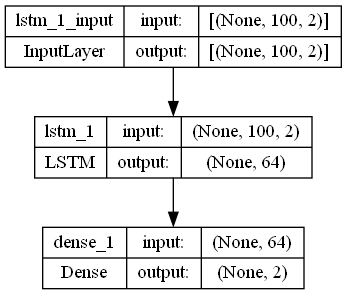
\includegraphics[width=0.4\linewidth]{Imagens/chap03/model_summary.png}
    \caption{Diagrama de blocos da rede neural desenvolvida. Fonte: Autor.}
    \label{fig:model_summary}
\end{figure}

\subsection{Hiperparâmetros do treinamento}
Os hiperparâmetros do treinamento da rede são:
\begin{enumerate}
    \item Número de épocas ($E$): Indica o número de iterações de treinamento da rede.
    \item Tamanho de batelada ($B$): Indica o número de amostras utilizada no treinamento em uma época.
    \item Taxa de validação ($V$): Indica a porcentagem do total de amostras usadas no treinamento que serão utilizadas como validação. 
\end{enumerate}
Para este trabalho, foi utilizado $E=50$, $B=32$ e $V=10\%$. O ajuste desses e dos demais hiperparâmetros foi realizado pelo \textit{script} \ref{code:tune_model}.

\section{Implementação do Controle MPC}
A figura \ref{fig:mpc_loop} ilustra a malha de controle MPC proposta neste trabalho. A rede LSTM é utilizada como o modelo preditivo que será usado pelo otimizador.

\newpage
\begin{figure}[hbt!]
    \centering
    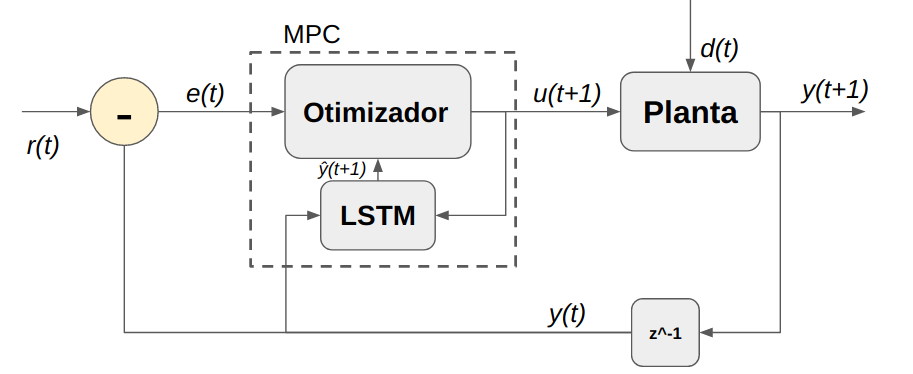
\includegraphics[width=0.8\linewidth]{Imagens/chap03/mpc_loop.png}
    \caption{Malha de controle MPC proposta neste trabalho. Fonte: Autor.}
    \label{fig:mpc_loop}
\end{figure}

\label{sec:mpc_imp}
\subsection{Modelo}
A predição realizada pela LSTM pode ser formulada como:
\begin{equation}
    \hat{y}(t) = g(U_H(t), Y_H(t-1))
\end{equation}
onde $U_H(t)= [u(t), u(t-1), ..., u(t-P+1)] \in \mathcal{R}^{P\times 2}$ é o vetor das entradas passadas e $Y_H(t)=[y(t), y(t-1), ... , y(t-Q+1)] \in \mathcal{R}^{Q \times 2}$ é o vetor de saídas passadas. Este modelo será utilizado dentro do otimizador para modelar as dinâmicas futuras do processo dentro de um horizonte de predição.

\subsection{Otimizador}
A otimização do controle NPMC em questão consiste na minimização de dois erros, o de rastreamento da saída e de regularização da variação de controle, como no exemplo formulado abaixo \cite{yan2022lstm}. A regularização é feita em cima da variação do sinal de controle e não do sinal original, pois é interessante minimizar grandes variações e sobressaltos nos parâmetros de entrada do processo GMAW, para evitar defeitos de fabricação.

\begin{align}
    \min_{U_F(t)} J(t) &= \min_{U_F(t)} a \sum_{k=1}^{N}(r(t+k)-\hat{y}(t+k))^2 + b \sum_{k=1}^{M}\Delta u(t+k)^2 \\
    \text{sujeito a} & \\
    &\hat{y}(t) = g(U_H(t), Y_H(t-1)) \\
    &u_{min} \leq u(t) \leq u_{max} \\
    &\hat{y}_{min} \leq \hat{y}(t) \leq \hat{y}_{max} \\
    & e(t+N) = 0  \\
    & \Delta u(k+M) = 0
\end{align}

onde $M$ e $N$ são os horizontes de controle e predição, respectivamente, $r(t)$ é a trajetória desejada, $a$ e $b$ são os pesos de saída e controle, respectivamente, $U_F(t) = [u(t+1), u(t+2), ... , u(t+M)] \in \mathcal{R}^{M \times 2}$ e $Y_F(t) = [y(t+1), y(t+2), ... , y(t+N)] \in \mathcal{R}^{N \times 2}$, e $\Delta u(t+k) = u(t+k) - u(t+k-1)$. Para instante $t$, calcula-se o controle ótimo $U^*_F(t)$ e utiliza como controle o primeiro ponto. Em suma $u^*(t) = U^*_F(0)$. 

Essa minimização é atingida através de um algoritmo de descida de gradiente (GD) que atualiza $U_F(t)$ de acordo com:

\begin{align}
    U_F^{k+1} &= U_F^k + \Delta U_F^k \\
    \Delta U_F^k &= \eta\left(\frac{\partial J^k}{\partial U_F^k}\right)
\end{align}

onde $\eta > 0$ é a taxa de atualização do otimizador. A Matriz Jacobiana é denotado por
\begin{align} \label{eq:dJdU}
    \frac{\partial J^k}{\partial U_F^k} &= \begin{bmatrix}
        \frac{\partial J}{\partial u(t+1)} \\
        ... \\
        \frac{\partial J}{\partial u(t+M)} 
    \end{bmatrix}
\end{align}

onde o $h$-ésimo elemento da matriz definida em \ref{eq:dJdU} é definido por 
\begin{align}\label{eq:dJdu}
    \frac{\partial J}{\partial u(t+h)} = &-2a\sum_{j=1}^N [r(t+j) - \hat{y}(t+j)] \frac{\partial \hat{y}(t+j)}{\partial u(t+h)} \\
    &+2b\sum_{j=1}^M \Delta u(t+j) \frac{\partial \Delta u(t+j)}{\partial u(t+h)}
\end{align}

O termo $\frac{\partial \Delta u(t+j)}{\partial u(t+h)}$ é expandido em termos da função Delta de Kronecker 
\begin{align}
    \frac{\partial \Delta u(t+j)}{\partial u(t+h)} &= \frac{\partial u(t+j)}{\partial u(t+h)} - \frac{\partial u(t+j-1)}{\partial u(t+h)} \\
    &= \delta(h,j) - \delta(h,j-1)
\end{align}
onde $\delta(h,j)=\begin{cases}
    1 & \text{se } h=j \\
    0 & \text{se } h \neq j
\end{cases}$. 

Já o termo $\frac{\partial \hat{y}(t+j)}{\partial u(t+h)}$ é extraído do modelo LSTM através de uma função própria da biblioteca do $tensorflow$ \cite{tensorflow2015} que calcula via \textit{Backpropagation Trough Time} (BPTT) \cite{lillicrap2019backpropagation}. O detalhamento do algoritmo de estimação de $\frac{\partial \hat{y}(t+j)}{\partial u(t+h)}$ e de $\frac{\partial J^k}{\partial U_F^k}$ estão descritos nos Algoritmos \ref{alg:bptt} e \ref{alg:compute_step}, respectivamente, e presentes no \textit{script} \ref{code:gmaw_mpc}
\newpage
\begin{algorithm}{
    \label{alg:bptt}
    \caption{Extração da matriz Jacobiana}
    \Entrada{$U_H$, $Y_H$, $U_F$}
    \Saida{Matriz Jacobiana $\frac{\partial \hat{y}(t+j)}{\partial u(t+h)}$ i $\in [1, N]$, $j \in [1, i]$}
    $k = 1$\;\\
    \While{k \leq M}{
        \If{$k < M$}{
            $u(t+k) = U_F(k)$\; \\
        }
        \Else{
            $u(t+k) = u(t+M)$
        }
        Atualiza $U_H(t+k)$ com $u(t+k)$\;
        $x = (U_H(t+k), Y_H(t))$\; \\
        Calcula $\hat{y}(t+k)$ por $g(x(t+k))$\; \\
        Extrai $\frac{\partial \hat{y}(t+k)}{x(t+k)}$\; \\
        $l = 1$\; \\
        \While{h \leq P}{
            $\frac{\partial \hat{y}(t+k)}{u(t+h)} = \frac{\partial \hat{y}(t+k)}{x(t+k)} (P-h) $\; \\
            $h = h+1$ \;
        }
        Atualiza $Y_H(t+k)$ com $\hat{y}(t+k)$\; \\
        $k = k + 1$\;
    }
}
\end{algorithm}

\newpage
\begin{algorithm}{
    \label{alg:compute_step}
    \caption{Otimização do controle $U_F$ via GD}
    \Entrada{$U_F(t)$, $R(t)$, $\frac{\partial \hat{y}(t+j)}{\partial u(t+h)}$ i $\in [1, N]$, $j \in [1, i]$, $a$, $b$ e $\eta$}
    \Saida{$U_F^{k+1}(t)$}
    Calcula $\Delta U_F(t) = [\Delta u_F(t+1), \Delta u_F(t+2), ... , \Delta u_F(t+M)]$\; \\
    Calcula $\frac{\partial \Delta U_F}{\partial U_F}$\;\\
    $j = 1$\; \\
    \While{j \leq M}{
        $\frac{\partial J}{\partial u(t+j)} = -2 \sum_{l=1}^2a_l\left(\sum_{k=1}^{N} [r(t+k)-\hat{y}(t+k)]\frac{\partial \hat{y}(t+k)}{\partial u(t+j)}\right) + 2 \sum_{l=1}^2b_l\left(\sum_{k=1}^{N} \Delta u_F(t+k)\frac{\partial \Delta u_F(t+k)}{\partial u(t+j)}\right)$\; \\
        $u(t+j)^{k+1} = u(t+j)^k -\eta \frac{\partial J}{\partial u(t+j)}$ \; \\
        $j = j + 1$\;
    }
}
\end{algorithm}

Daí, roda-se a simulação utilizando $a=[10,10]$, $b=[1, 1]$, $M=P$, $N=Q$, $\eta=0.1$ e 10 passos de otimização. O algoritmo \ref{alg:mpc_algo} é encarregado da simulação do controle MPC.
\begin{algorithm}{
    \label{alg:mpc_algo}
    \caption{Simulação do controle MPC}
    \Entrada{$R(t)$, $M$, $N$, $a$, $b$, $\eta$, $y(0)$, o tempo total de simulação $T$, a tolerância $\epsilon_{opt}$}
    \Saida{$U^*(t)$}
    Inicializa $Y_H$ e $U_H$\; \\
    Atualiza $Y_H$ com $y(0)$\; \\
    \While{t \leq T}{
        Roda o Algoritmo 1 para extrair $U_F(0)$ e $Y_F(0)$\; \\
        $u^*(1)=u_F(1)$ \; \\
        Atualiza $U_F$ com $u^*(1)$\; \\
        Calcula $y(1)$ através do modelo dinâmico equacionado \; \\
        Atualiza $Y_H$ com $y(1)$\; \\
        $t = t + 1$\; \\
    }
}
\end{algorithm}

\newpage
\subsection{Análise de Estabilidade}
Em geral, garantir a estabilidade de um sistema de controle é de suma importância dentro da teoria de controle. No caso deste trabalho, onde o controle preditivo é realizado através de uma rede neural que modela uma dinâmica não linear (LSTM-NMPC), a estabilidade é investigada checando a monotonicidade da função custo estabelecida, que garante a estabilidade asintótica do controlador.

Assumindo que $U_F(k)$ é ótimo no tempo $k$, estimado pelo otimizador. Agora, introduzindo um controle subótimo $U_Fk+1)$ postulado no tempo $k+1$:
\begin{equation}
    U_F(k+1) = [u(k+1), u(k+2), ... , u(k+M)]^T
\end{equation}

cuja função custo é definida como
\begin{equation}
        \min_{U_F(k+1)} J(k+1) &= \min_{U_F(k+1)} a \sum_{j=1}^{N}(r(k+1+j)-\hat{y}(k+1+j))^2 + b \sum_{j=1}^{M}\Delta u(k+1+j)^2
\end{equation}

\newpage
Com isso, a diferença entre $J(k)$ e $J(k+1)$ é
\begin{align}
    J(k+1) - J(k) &= a[e^2(k+N+1)-e^2(k+1)] - b\Delta u^2(k) = \\
    &= -ae^2(k+1) - b\Delta u^2(k) \leq 0
\end{align}

Portanto, para $a, b > 0$, o custo $J(k)$ é decai monotonicamente com respeito ao tempo e o controle é estável. 

\chapter{Resultados e Discussão}
\label{chap4}
\section{Geração dos Dados}
\subsection{Simulação}
A figura \ref{fig:sim_inputs_raw} ilustra os sinais de entrada ($f$ e $I_r$) de treino e teste da simulação, utilizando os valores descritos na tabela \ref{tab:params_aprbs}:

\begin{figure}[hbt!]
    \centering
    \includegraphics[width=0.8\linewidth]{Imagens/chap04/sim_inputs_train_raw.png}
    \hfill
    \includegraphics[width=0.8\linewidth]{Imagens/chap04/sim_inputs_test_raw.png}
    \caption{Sinais de entrada de treino (acima) e teste (abaixo) da simulação do sistema. O sinal foi truncado em 100 amostras para facilitar a visualização. Fonte: Autor}
    \label{fig:sim_inputs_raw}
\end{figure}

A figura \ref{fig:sim_outputs_raw} ilustra os sinais de saída ($w_e$ e $h$) de treino e teste da simulação

\begin{figure}[hbt!]
    \centering
    \includegraphics[width=0.8\linewidth]{Imagens/chap04/sim_outputs_train_raw.png}
    \hfill
    \includegraphics[width=0.8\linewidth]{Imagens/chap04/sim_outputs_test_raw.png}
    \caption{Saídas de saída de treino (acima) e teste (abaixo) da simulação. O sinal foi truncado em 100 amostras para facilitar a visualização. Fonte: Autor}
    \label{fig:sim_outputs_raw}
\end{figure}

\subsection{Dados experimentais}
A figura \ref{fig:exp_inputs_raw} ilustra a entrada $f$ de treino e teste dos dados experimentais:
\begin{figure}[hbt!]
    \centering
    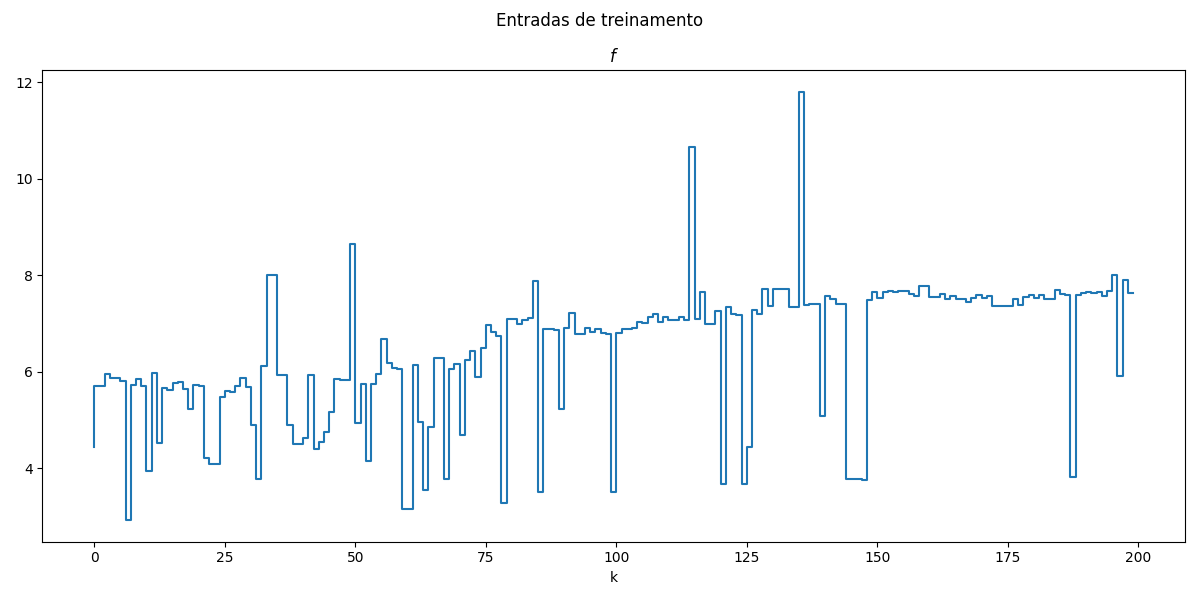
\includegraphics[width=0.8\linewidth]{Imagens/chap04/experiment_inputs_train_raw.png}
    \hfill
    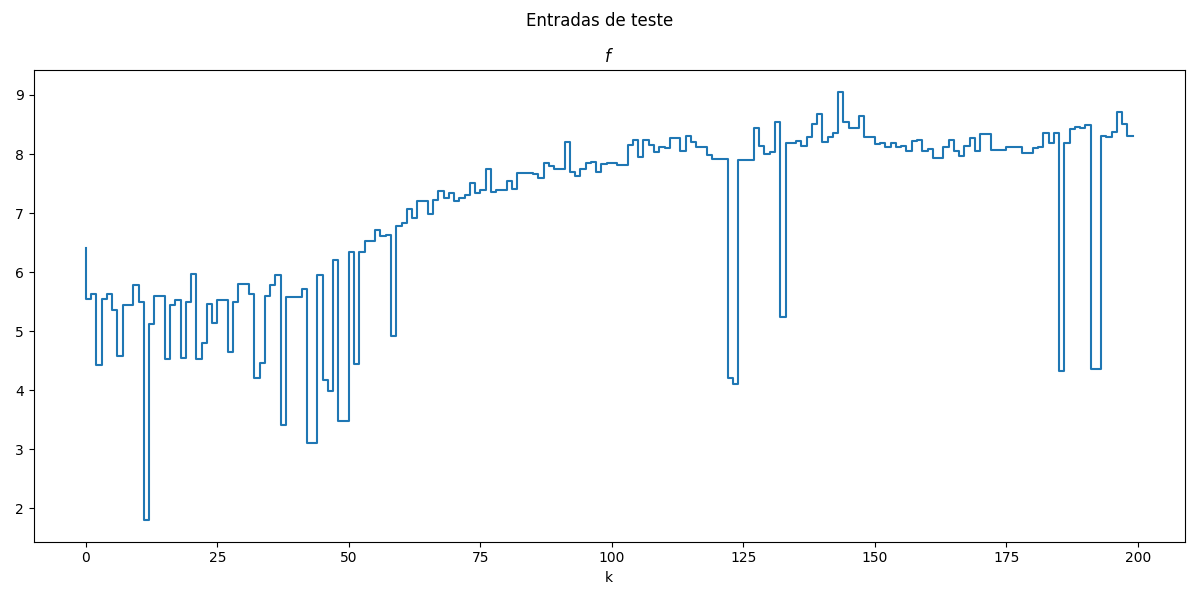
\includegraphics[width=0.8\linewidth]{Imagens/chap04/experiment_inputs_test_raw.png}
    \caption{Entrada de treino (acima) e teste (abaixo) dos dados experimentais. Fonte: Autor}
    \label{fig:exp_inputs_raw}
\end{figure}

A figura \ref{fig:exp_outputs_raw} ilustra a saída $w_e$ de treino e teste dos dados experimentais:
\begin{figure}[hbt!]
    \centering
    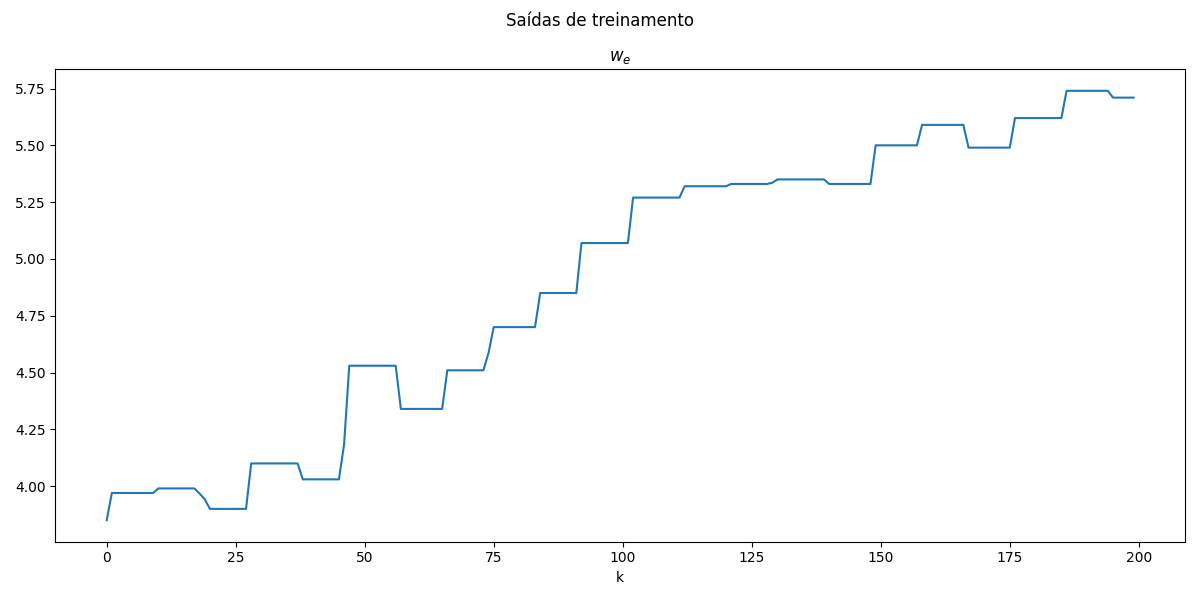
\includegraphics[width=0.8\linewidth]{Imagens/chap04/experiment_outputs_train_raw.png}
    \hfill
    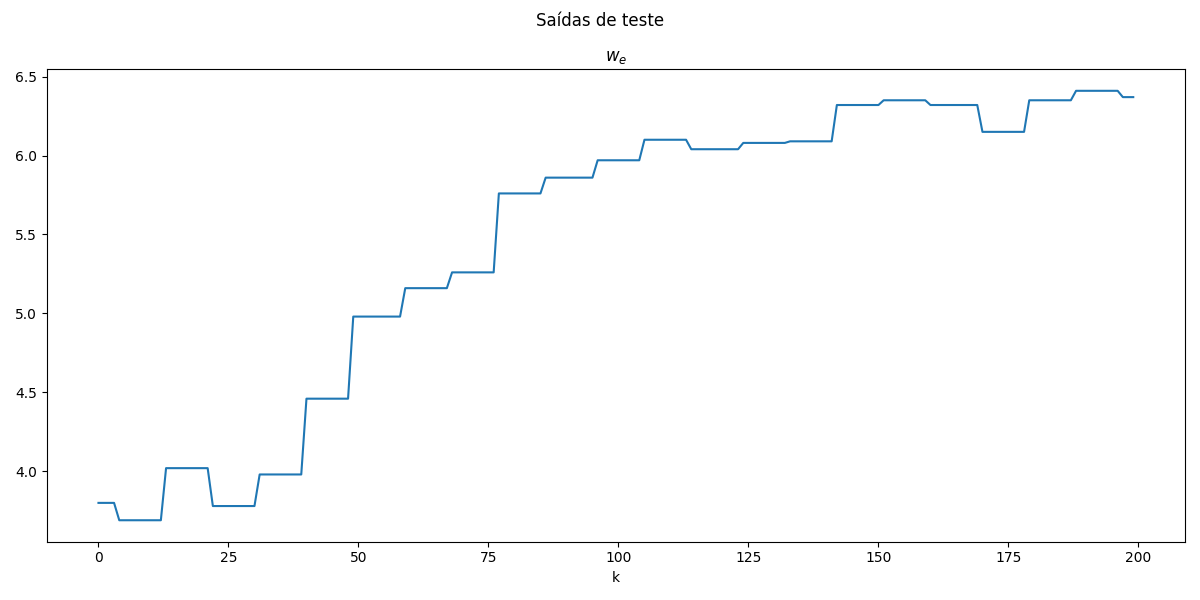
\includegraphics[width=0.8\linewidth]{Imagens/chap04/experiment_outputs_test_raw.png}
    \caption{Saída de treino (acima) e teste (abaixo) dos dados experimentais. Fonte: Autor}
    \label{fig:exp_outputs_raw}
\end{figure}

\newpage
\section{Tratamento dos Dados}
\subsection{Simulação}
As figuras \ref{fig:sim_inputs} e \ref{fig:sim_outputs} ilustram a normalização min-max e média-desvio padrão, respectivamente, das entradas e saídas do processo.

\begin{figure}[hbt!]
    \centering
    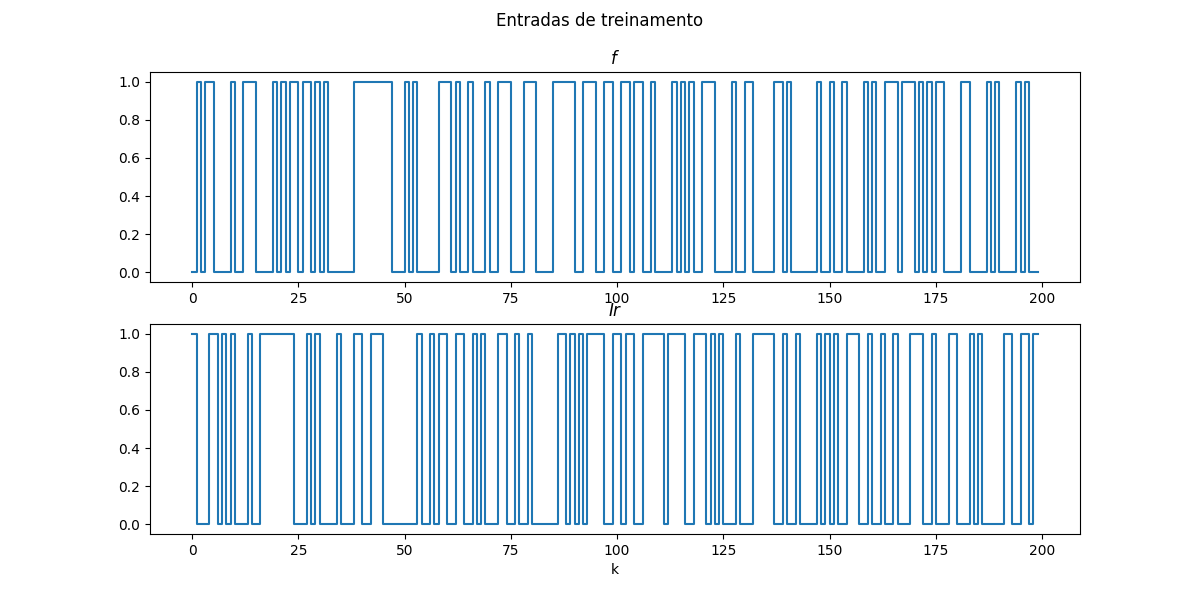
\includegraphics[width=0.8\linewidth]{Imagens/chap04/simulation_inputs_train.png}
    \hfill
    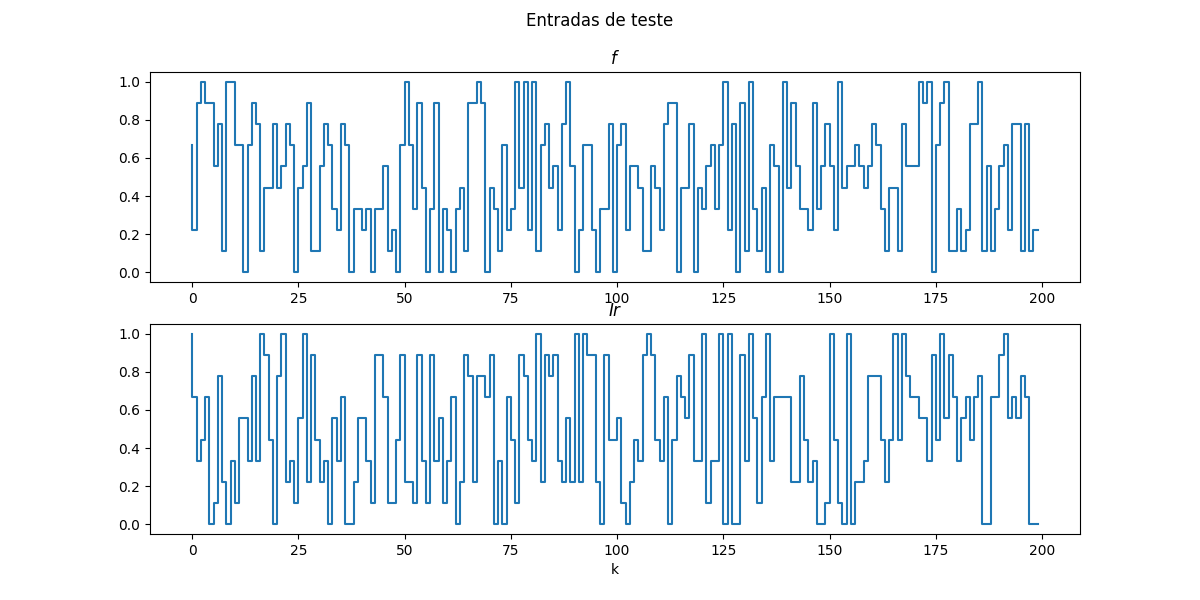
\includegraphics[width=0.8\linewidth]{Imagens/chap04/simulation_inputs_test.png}
    \caption{Sinais normalizados de treino (cima) e teste (baixo) utilizados como entrada da simulação do sistema.
 O sinal foi truncado em 100 amostras para facilitar a visualização. Fonte: Autor}
    \label{fig:sim_inputs}
\end{figure}

\begin{figure}[hbt!]
    \centering
    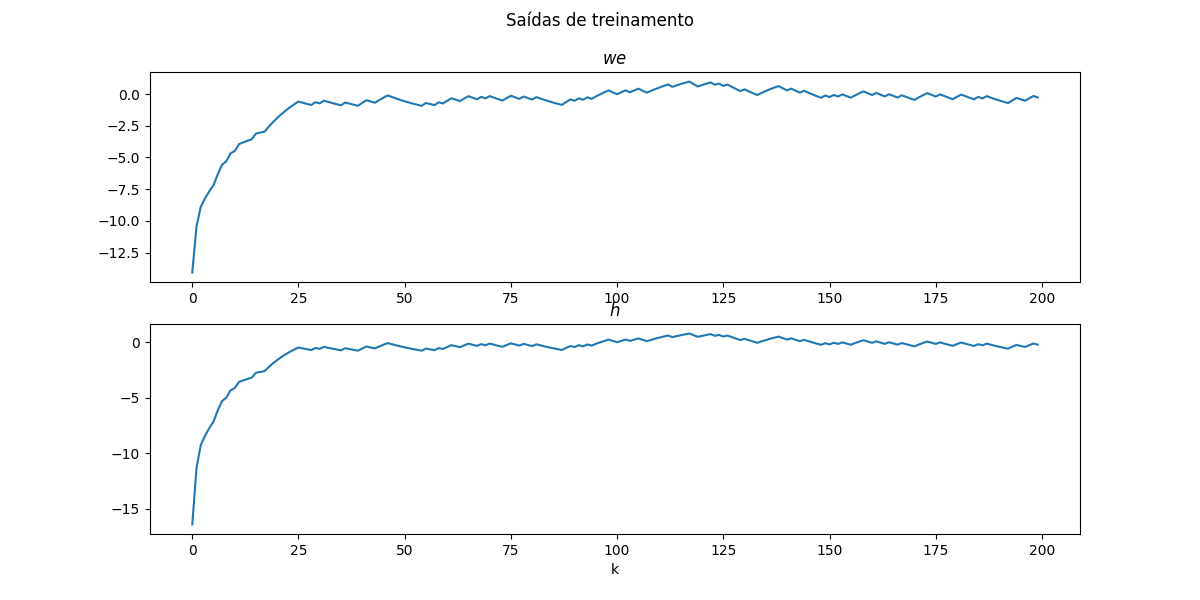
\includegraphics[width=0.8\linewidth]{Imagens/chap04/simulation_outputs_train.png}
    \hfill
    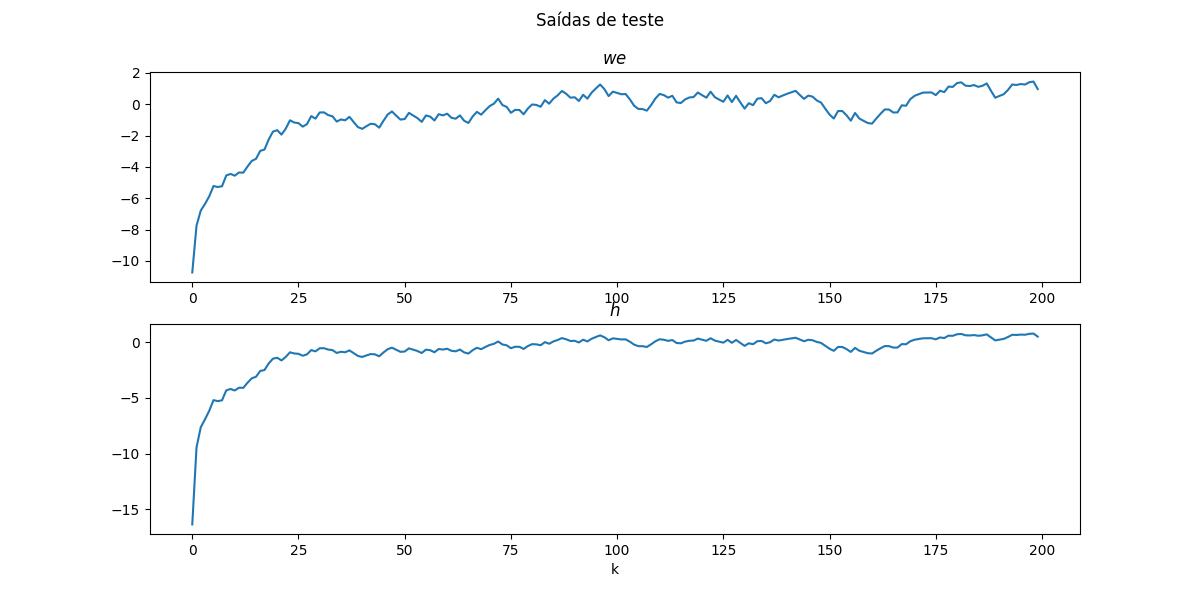
\includegraphics[width=0.8\linewidth]{Imagens/chap04/simulation_outputs_test.png}
    \caption{Saídas normalizadas de treino (cima) e teste (baixo) da simulação. O sinal foi truncado em 100 amostras para facilitar a visualização. Fonte: Autor}
    \label{fig:sim_outputs}
\end{figure}

\subsection{Dados experimentais}
As figuras \ref{fig:exp_inputs} e \ref{fig:exp_outputs} ilustram a normalização min-max e média-desvio padrão, respectivamente, das entradas e saídas dos dados experientais.

\begin{figure}[hbt!]
    \centering
    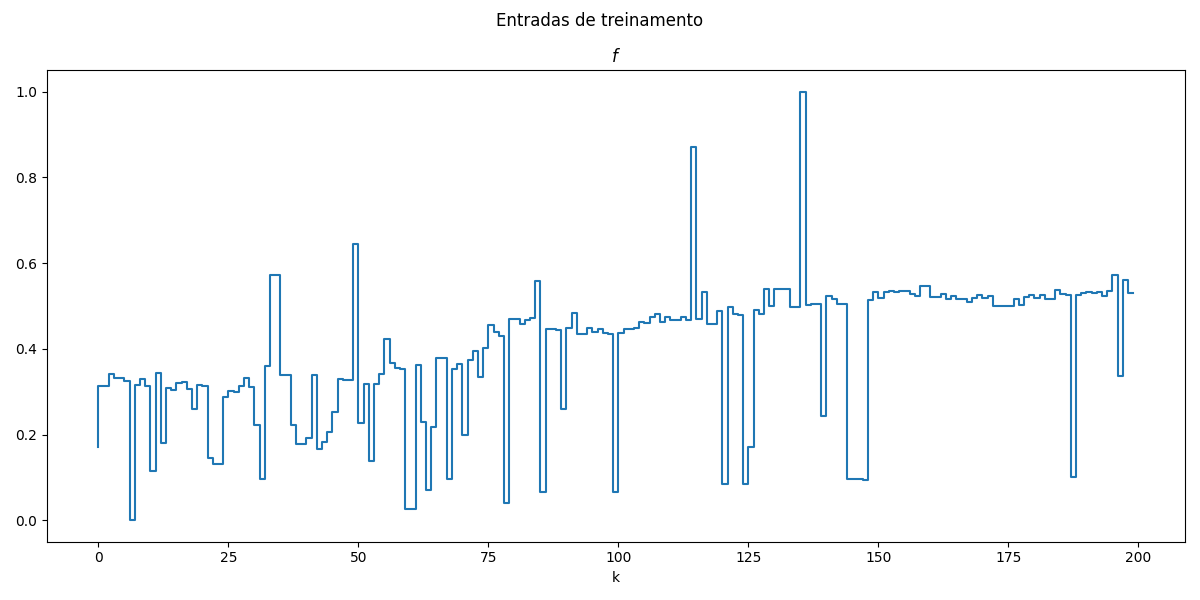
\includegraphics[width=0.8\linewidth]{Imagens/chap04/experiment_inputs_train.png}
    \hfill
    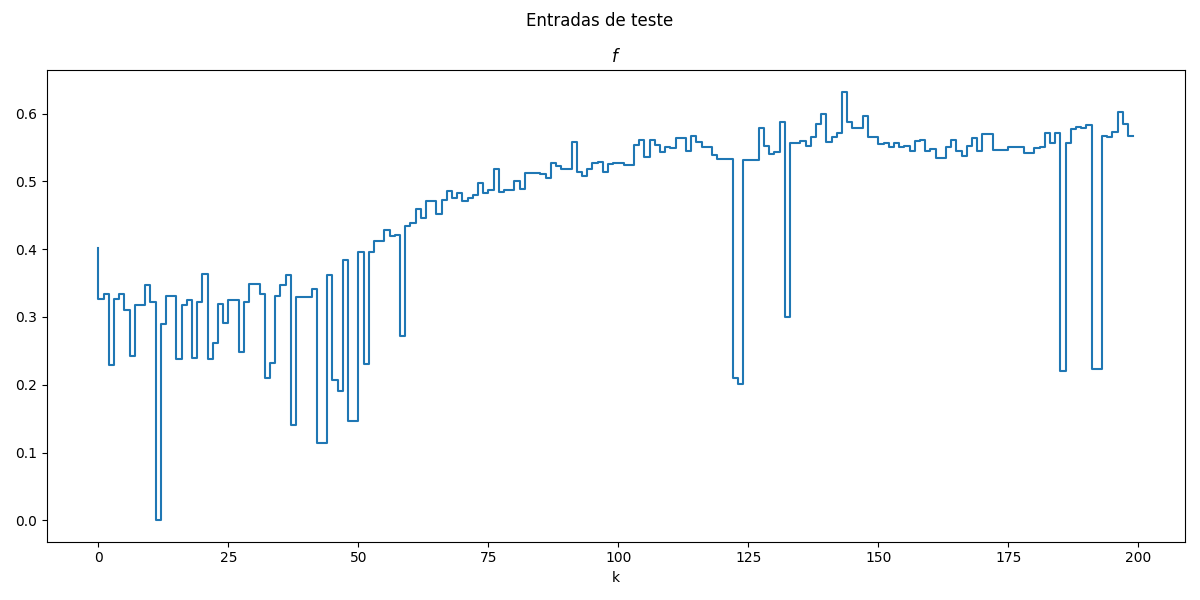
\includegraphics[width=0.8\linewidth]{Imagens/chap04/experiment_inputs_test.png}
    \caption{Sinais normalizados de treino (cima) e teste (baixo) de entrada dos dados experimentais.
 O sinal foi truncado em 100 amostras para facilitar a visualização. Fonte: Autor}
    \label{fig:exp_inputs}
\end{figure}

\begin{figure}[hbt!]
    \centering
    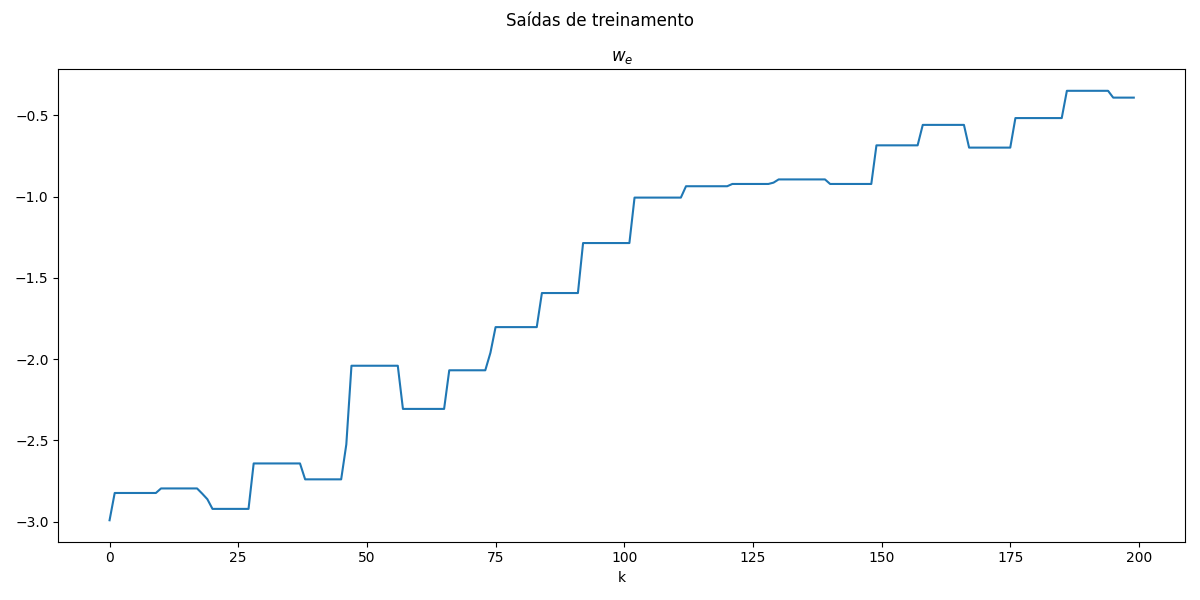
\includegraphics[width=0.8\linewidth]{Imagens/chap04/experiment_outputs_train.png}
    \hfill
    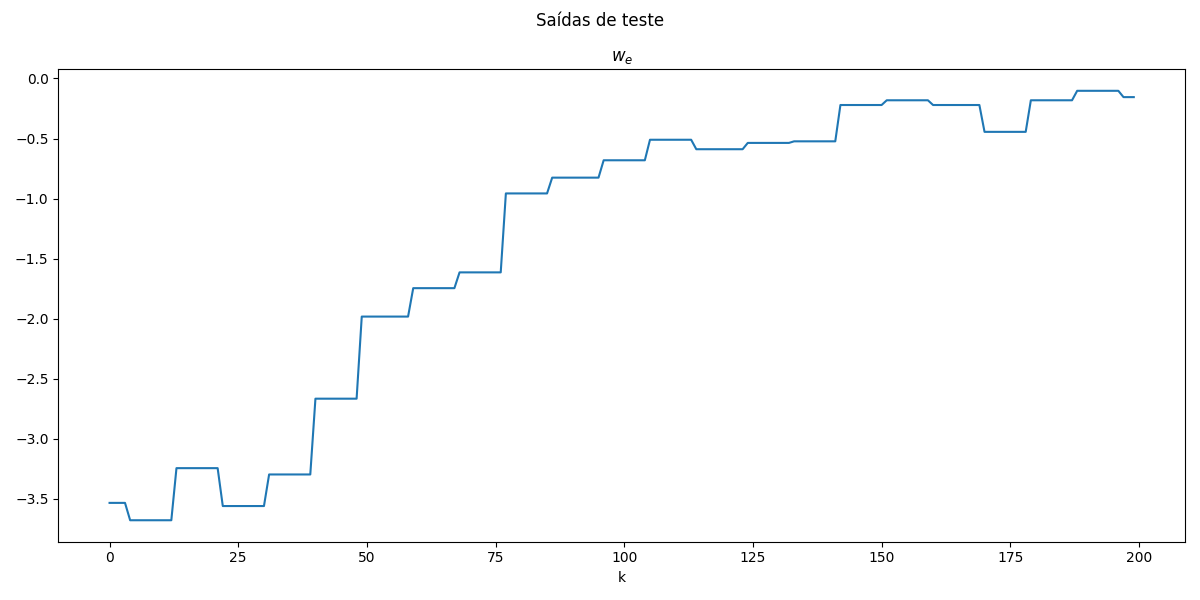
\includegraphics[width=0.8\linewidth]{Imagens/chap04/experiment_outputs_test.png}
    \caption{Sinais normalizados de treino (cima) e teste (baixo) de saída dos dados experimentais.
    \label{fig:exp_outputs}
\end{figure}

\section{Modelagem da rede LSTM}
\subsection{Ajuste dos hiperparâmetros}
\subsubsection{Simulação}
As figuras \ref{fig:sim_hp_metrics} ilustram os resultados do treinamento dos hiperparâmetros $P$, $Q$ e tamanho de batelada.

\begin{figure}[hbt!]
    \centering
    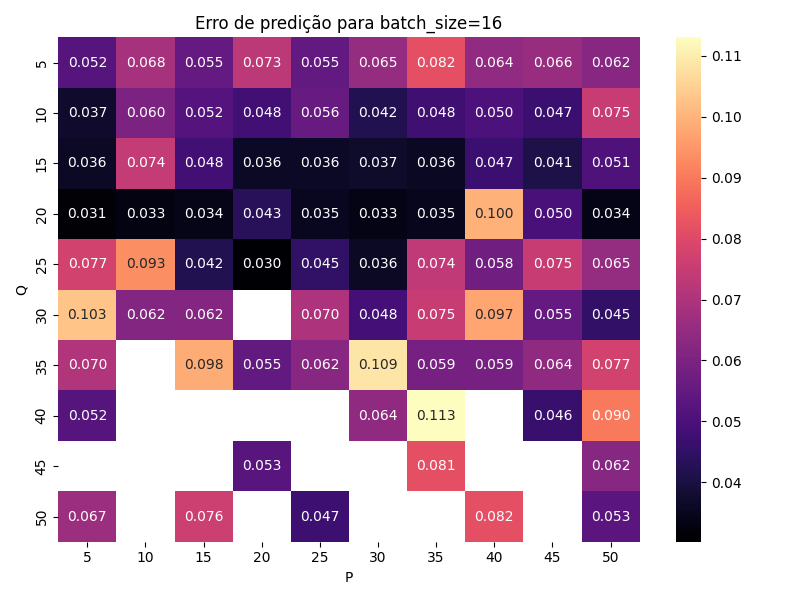
\includegraphics[width=0.7\linewidth]{Imagens/chap04/simulation_hp_metrics_16.png}
    \hfill
    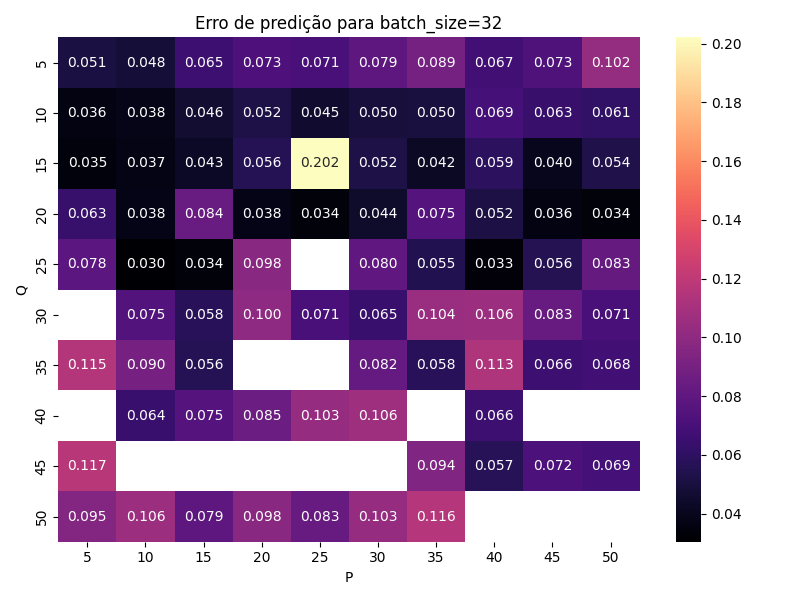
\includegraphics[width=0.7\linewidth]{Imagens/chap04/simulation_hp_metrics_32.png}
    \hfill
    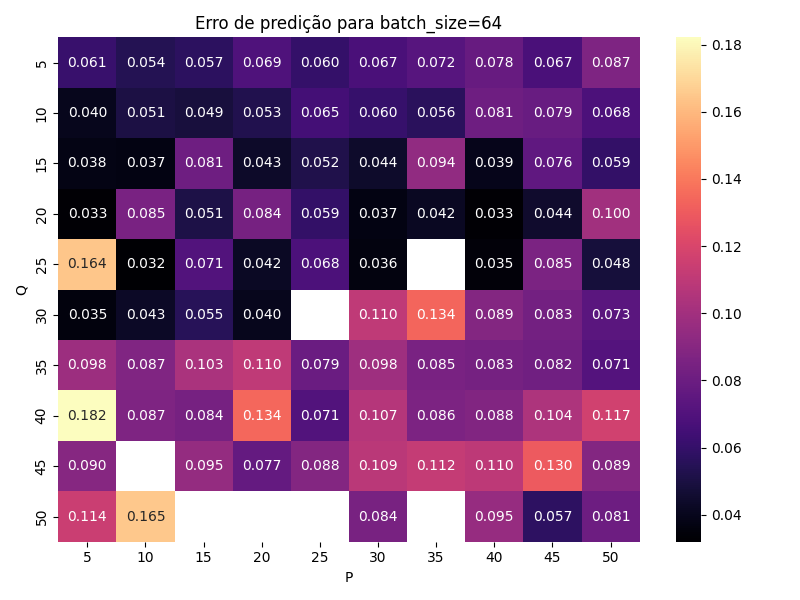
\includegraphics[width=0.7\linewidth]{Imagens/chap04/simulation_hp_metrics_64.png}
    \caption{Mapa de calor indicando o erro RMS para diferentes valores de $P$ e $Q$ e para tamanho de batelada 16 (esquerda), 32 (direita) e 64 (baixo). Fonte: Autor}
    \label{fig:sim_hp_metrics}
\end{figure}

O melhor resultado é o de $(P,Q,batch\_size)=(20,25,16)$, cujo RMSE é de 0.03.  Porém, a rede com hiperparâmetros $(P,Q,batch\_size)=(5,20,16)$ performou quase tão bem, como RMSE de 0.031, e utiliza uma janela significante menor de pontos históricos de entrada (5) e saída (20). Isso significa que o número de parâmetros dessa rede é inferior, o que acelera seu treinamento, portanto foi a rede escolhida. Os valores vazios são de treinamentos que retornaram um erro que é um outlier e foram removidos para auxiliar na visualização do mapa de calor. 

\subsubsection{Dados experimentais}
As figuras \ref{fig:exp_hp_metrics} ilustram os resultados do treinamento dos hiperparâmetros $P$, $Q$ e tamanho de batelada.

\begin{figure}[hbt!]
    \centering
    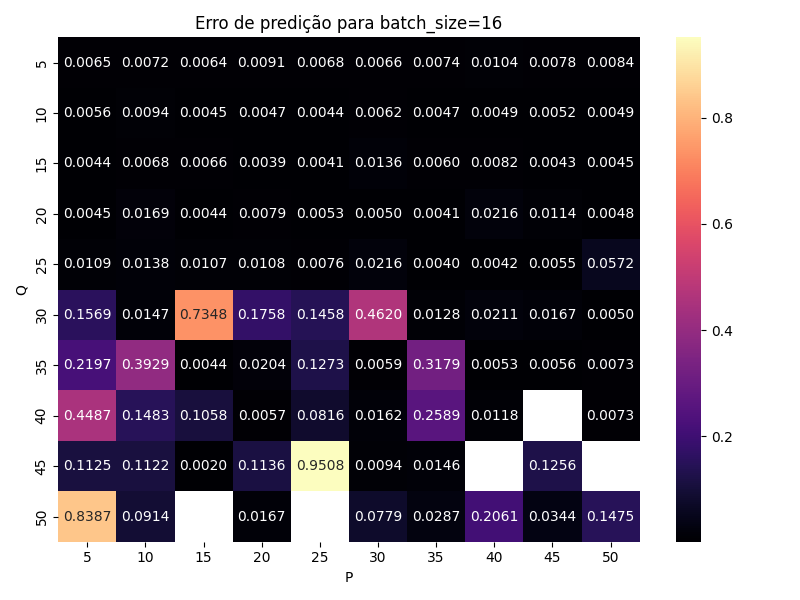
\includegraphics[width=0.7\linewidth]{Imagens/chap04/experiment_hp_metrics_16.png}
    \hfill
    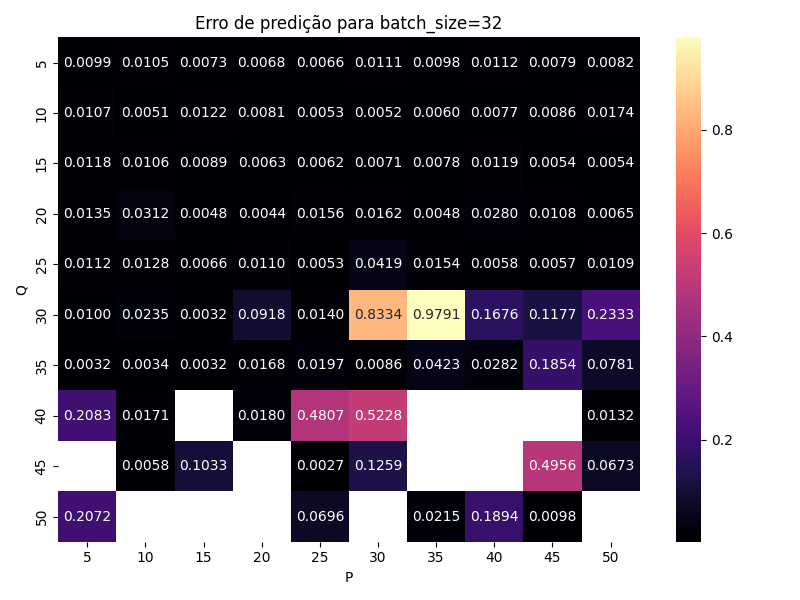
\includegraphics[width=0.7\linewidth]{Imagens/chap04/experiment_hp_metrics_32.png}
    \hfill
    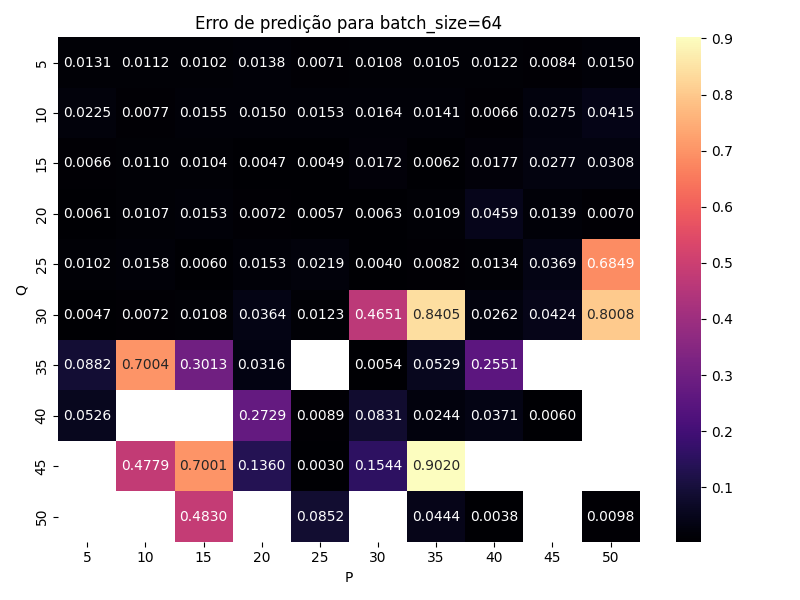
\includegraphics[width=0.7\linewidth]{Imagens/chap04/experiment_hp_metrics_64.png}
    \caption{Mapa de calor indicando o erro RMS para diferentes valores de $P$ e $Q$ e para tamanho de batelada 16 (esquerda), 32 (direita) e 64 (baixo). Fonte: Autor}
    \label{fig:exp_hp_metrics}
\end{figure}

O melhor resultado é o de $(P,Q,batch\_size)=(15,45,16)$, cujo RMSE é de 0.002. A predição dos modelos escolhidos estão descritas abaixo.

\subsection{Predição}
\subsubsection{Simulação}
A figura \ref{fig:lstm_prediction} mostra a predição das saídas do processo utilizando esta rede, num horizonte de 1000 pontos.
\begin{figure}[hbt!]
    \centering
    \includegraphics[width=0.7\linewidth]{Imagens/chap04/simulation_lstm_prediction.png}
    \caption{Predição das duas saídas do processo GMAW utilizando a rede com hiperparâmetros $P=20$, $Q=25$ e tamanho de batelada 16. Fonte: Autor}
    \label{fig:sim_lstm_prediction}
\end{figure}

A performance da rede é extremamente satisfatória, mostrando que foi capaz de modelar o processo e que se torna necessário interessante modificar a modelagem do distúrbio. Na figura \ref{fig:sim_error_histogram} está contido o histograma do erro de predição de cada saída, com a respectiva média, desvio padrão e p-valor do teste de normalidade. 

\begin{figure}[hbt!]
    \centering
    \includegraphics[width=0.7\linewidth]{Imagens/chap04/simulation_error_histogram.png}
    \caption{Histograma do erro de predição de cada saída, indicando a média, desvio padrão e valor-p do teste de normalidade Shapiro \cite{shapiro1965analysis}. Fonte: Autor.}
    \label{fig:sim_error_histogram}
\end{figure}

Nota-se que, para ambas as saídas, o ruído de predição é normal e de média próxima a zero, indicando que o modelo foi bem sucedido em modelar o processo dinâmico em questão.

\subsubsection{Dados experimentais}
A figura \ref{fig:lstm_prediction} mostra a predição das saídas do processo utilizando esta rede, num horizonte de 1000 pontos.
\begin{figure}[hbt!]
    \centering
    \includegraphics[width=0.7\linewidth]{Imagens/chap04/simulation_lstm_prediction.png}
    \caption{Predição das duas saídas do processo GMAW utilizando a rede com hiperparâmetros $P=20$, $Q=25$ e tamanho de batelada 16. Fonte: Autor}
    \label{fig:sim_lstm_prediction}
\end{figure}

A performance da rede é extremamente satisfatória, mostrando que foi capaz de modelar o processo e que se torna necessário interessante modificar a modelagem do distúrbio. Na figura \ref{fig:sim_error_histogram} está contido o histograma do erro de predição de cada saída, com a respectiva média, desvio padrão e p-valor do teste de normalidade. 

\begin{figure}[hbt!]
    \centering
    \includegraphics[width=0.7\linewidth]{Imagens/chap04/simulation_error_histogram.png}
    \caption{Histograma do erro de predição de cada saída, indicando a média, desvio padrão e valor-p do teste de normalidade Shapiro \cite{shapiro1965analysis}. Fonte: Autor.}
    \label{fig:sim_error_histogram}
\end{figure}

Nota-se que, para ambas as saídas, o ruído de predição é normal e de média próxima a zero, indicando que o modelo foi bem sucedido em modelar o processo dinâmico em questão.


\section{Controle MPC}
As figuras \ref{fig:mpc_inputs} e \ref{fig:mpc_outputs} ilustram os sinais de controle otimizados via MPC e as saídas controladas, respectivamente. 

\newpage
\begin{figure}[hbt!]
    \centering
    \includegraphics[width=0.7\linewidth]{Imagens/chap04/mpc_inputs.png}
    \caption{Sinais de controle via MPC. Fonte: Autor.}
    \label{fig:mpc_inputs}
\end{figure}

\begin{figure}[hbt!]
    \centering
    \includegraphics[width=0.7\linewidth]{Imagens/chap04/mpc_outputs.png}
    \caption{Saías controladas pelo MPC. Fonte: Autor.}
    \label{fig:mpc_outputs}
\end{figure}

A implementação foi capaz de controlar as saídas em torno de um referencial determinado. A oscilação de controle e saída estão dentro do aceitável considerando os limites físicos do processo. A tabela \ref{tab:metrics_mpc} descreve as métricas do controle do processo.

\newpage
\begin{table}[hbt!]
    \centering
    \begin{tabular}{c c c c}
         \hline
         Saída & Overshoot (\%) & RMSE & \Delta \bar{u} / u_{max} (\%) \\
         \hline
         $w_e$ & 12.82 & 6.28 \cdot 10^{-9} & 1.8\\
         $h$ & 8.14 & 7.23 \cdot 10^{-11} & 1.4 \\
         \hline
    \end{tabular}
    \caption{Métricas de controle MPC do processo GMAW estabalecido}
    \label{tab:metrics_mpc}
\end{table}
\chapter{Conclusões}
\label{chap6}
Com o intuito de lidar com um problema de controle multivariável de um processo GMAW, que possui dinâmica não linear, este trabalho propôs um controle preditivo (MPC) baseado em DL (LSTM-NMPC).

Primeiramente, foi realizada a simulação do processo GMAW, utilizando as equações dinâmicas de \cite{bendia2021multivariable}, e os dados foram tratados usando a normalização e padronização das entradas e saídas.

Depois, uma RN baseada na arquitetura LSTM foi treinada com o intuito de modelar o processo GMAW, ajustando-se os seus hiperparâmetros através da busca em grade.

Por fim, o melhor modelo foi utilizado dentro do MPC para otimizar o controle da geometria do cordão através de um algoritmo de GD adaptativo. O controle proposto foi provado estável, através de análise teórica.

O framework do MPC desenvolvido neste trabalho pode ser usado para se comunicar com o robô através do protocolo de comunicação do ROS.

O framework do MPC desenvolvido neste trabalho pode ser aplicado para qualquer controle preditivo de um processo não linear, apenas refazendo o treinamento com uma nova base de dados específica.


\backmatter
%\nocite{*}
\printbibliography
% \appendix
% \chapter{Códigos desenvolvidos}
\label{appendice}
\section{Dinâmica do processo GMAW}\label{code:gmaw_process}
Código \textit{gmaw\_process.py}:
{\small \lstinputlisting{code/gmaw_process.py}}


\section{Geração dos dados}\label{code:generate_database}
Código \textit{generate\_database.py}:
{\small \lstinputlisting{code/generate_database.py}}

\section{Processamento dos dados}\label{code:process_data}
Código \textit{process\_data.py}:
{\small \lstinputlisting{code/process_data.py}}

\section{Definição da Rede LSTM}\label{code:lstm}
Código \textit{lstm.py}:
{\small \lstinputlisting{code/lstm.py}}

\newpage

\section{Avaliação da rede LSTM}\label{code:evaluate_model}
Código \textit{evaluate\_model.py}:
{\small \lstinputlisting{code/evaluate_model.py}}

\section{Ajuste dos hiperparâmetros da rede LSTM}\label{code:tune_model}
Código \textit{tune\_model.py}:
{\small \lstinputlisting{code/tune_model.py}}

\section{Controle MPC do processo GMAW}\label{code:gmaw_mpc}
Código \textit{gmaw\_mpc.py}:
{\small \lstinputlisting{code/gmaw_mpc.py}}

\end{document}
